\documentclass{report}
\usepackage[utf8]{inputenc}
\usepackage[italian]{babel}
\usepackage{amsmath}
\usepackage{graphicx}
\usepackage{float}
\usepackage{pdfpages}
\usepackage{siunitx}
\usepackage{caption}
\usepackage{subcaption}
\usepackage{tikz}
\usetikzlibrary{shapes,arrows}

\DeclareSIUnit{\rpm}{rpm}
\sisetup{range-phrase=\div}

\title{Progetto no-brim}
\author{Daniele Moser, Francesco Maraner, Michele Mattè}



\begin{document}
\maketitle
\tableofcontents

\chapter{Introduzione}
no-brim è il progetto di una segatrice per tubi in PVC o altri materiali plastici, creato per il corso di Alta Formazione Professionale. Alla base di questo progetto, è presente la progettazione meccanica, elettronica e di programmazione di un macchinario semiautomatico per il taglio di lunghezza variabile di tubi mediante una discreta varietà di componenti (motori elettrici, assi, pistoni pneumatici, elettrovalvole, trasmissione a cinghia e lama circolare) che operano simultaneamente per realizzare il prodotto finale. Le motivazioni che ci hanno proiettato su questa tipologia di progetto derivano dal desiderio di mettere in atto le nozioni apprese durante il primo e secondo praticantato, dove ognuno dei 3 componenti del gruppo ha avuto modo di confrontarsi con il mondo del lavoro e di migliorare e accrescere le sue conoscenze nei vari ambiti in cui ha potuto lavorare, come la creazione di sistemi di trasmissione del moto o la programmazione.
\chapter{Meccanica}

\section{Descrizione macchina e motivazione dei componenti}
La parte meccanica, realizzata su Inventor, è stata divisa in 2 gruppi principali:
\begin{itemize}
\item Trasporto;
\item Taglio ed espulsione.
\end{itemize}

\subsection{Trasporto}
\begin{figure}[H]
  \centering
  \begin{subfigure}[H]{0.45\textwidth}
    \centering
    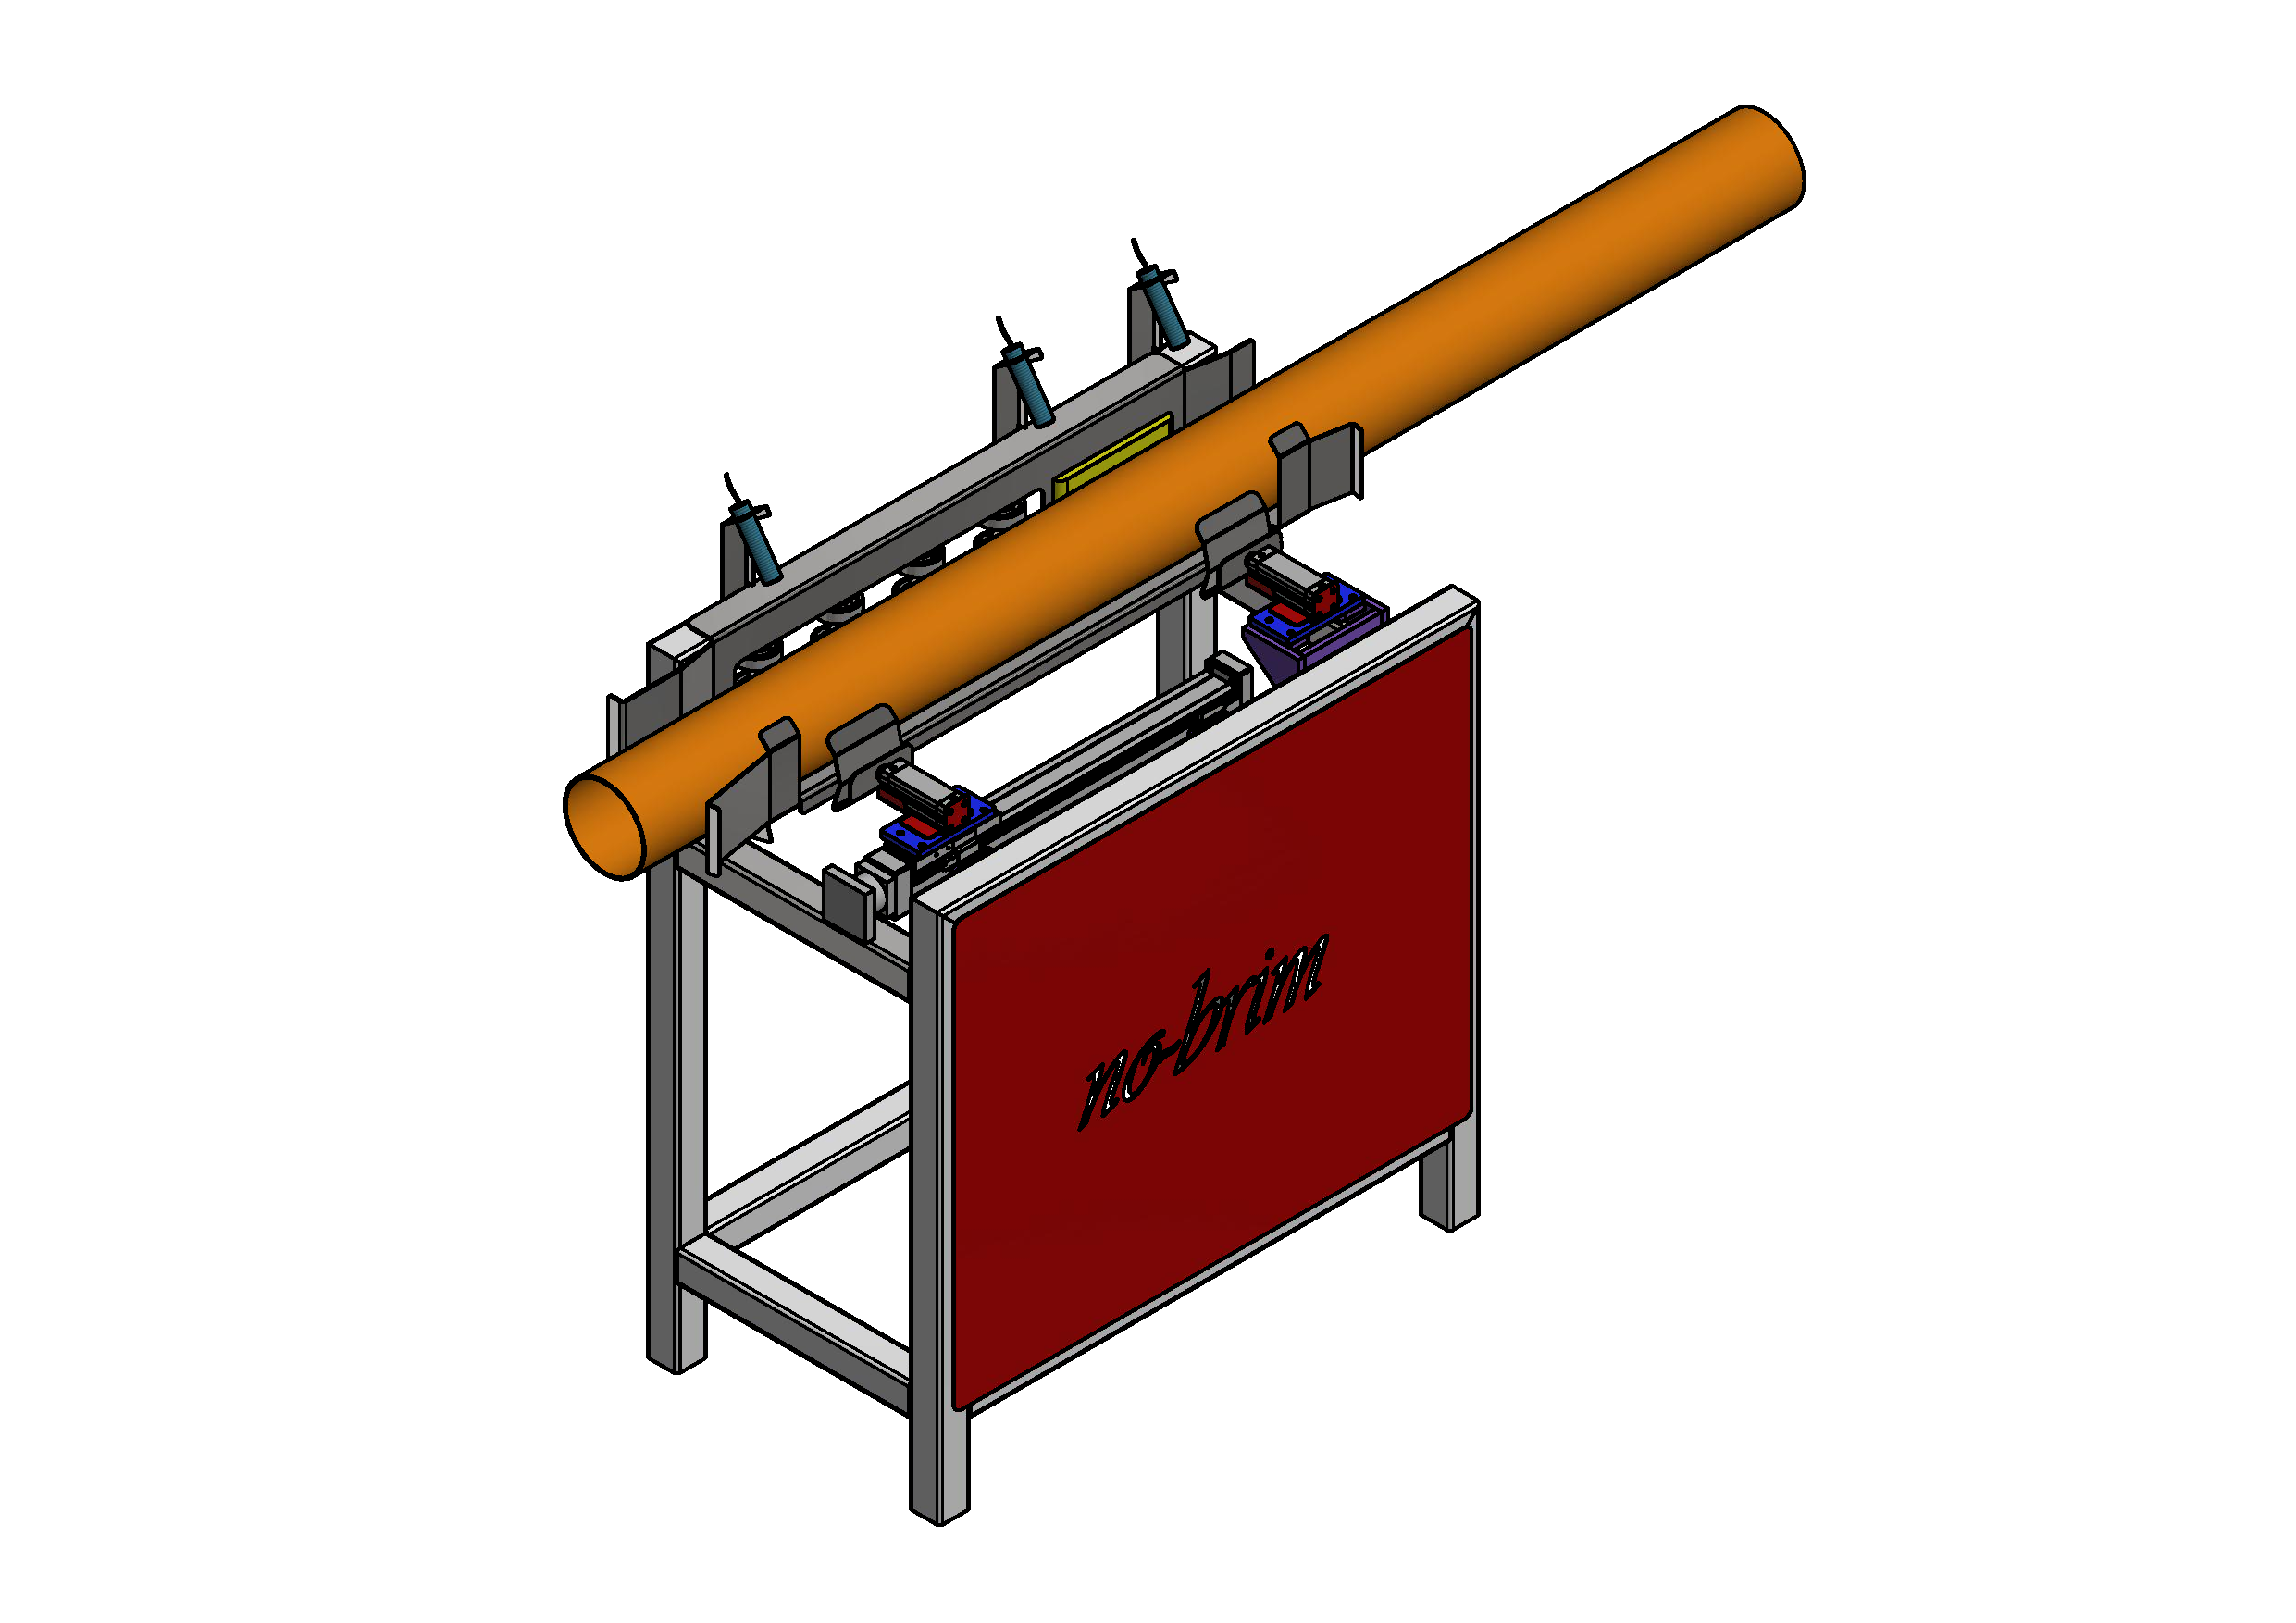
\includegraphics[width=\textwidth]{src/img/trasporto_1.pdf}
  \end{subfigure}
  \hfill
  \begin{subfigure}[H]{0.45\textwidth}
    \centering
    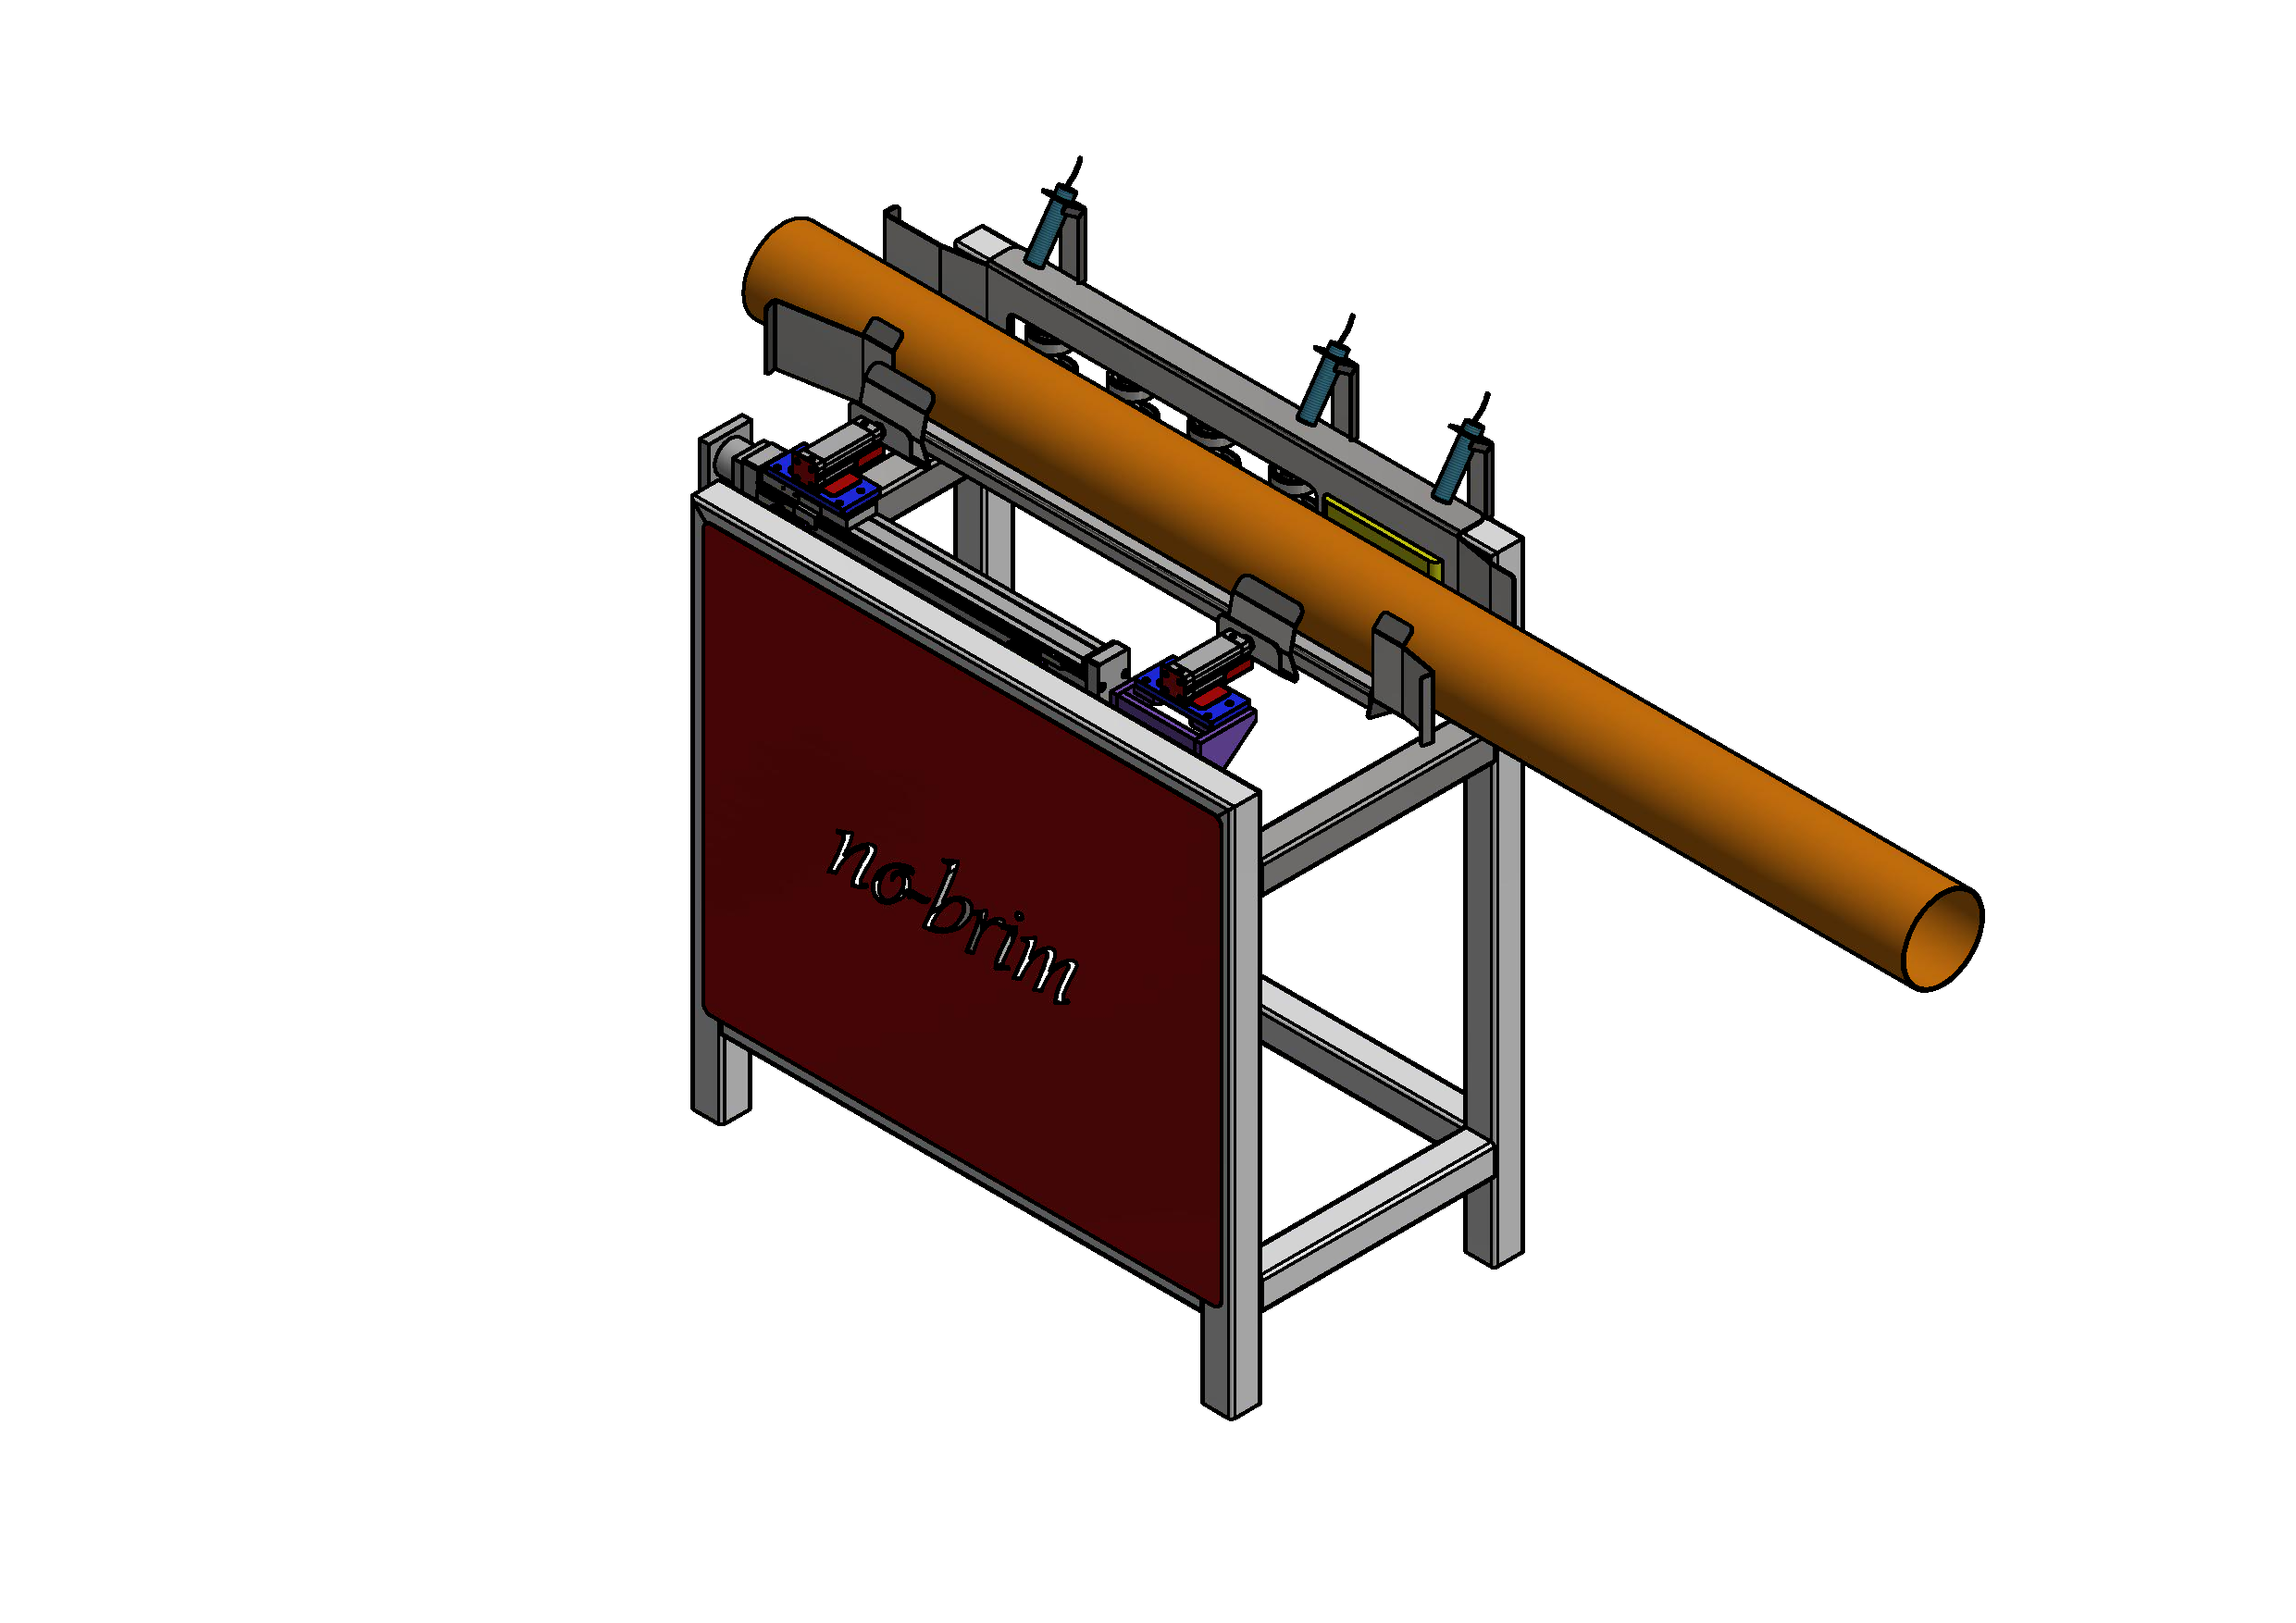
\includegraphics[width=\textwidth]{src/img/trasporto_2.pdf}
    \end{subfigure}
    \caption{Gruppo trasporto}
    \label{fig:vtcons}
\end{figure}
La prima parte si occupa del trasporto del tubo mediante un asse lineare ($l=\SI{300}{\mm}$) che sfrutta una trasmissione a vite a ricircolo di sfere, comandata da un motore elettrico, per spostare un pistone pneumatico (1M1), dove alla sua estremità è montata una lamiera che con la sua elasticità garantisce la corretta aderenza al tubo, sfruttando tutta la forza del pistone. Il pistone è stato collegato al pattino dell’asse lineare mediante una lamiera e una piastra. Dalla parte opposta all’asse, troviamo una lamiera a forma di “V” che garantisce il corretto scorrimento del tubo fino alla parte di taglio, grazie all’utilizzo di una rulliera costruita con dei cuscinetti a sfera.
Poco più a destra dell’asse lineare si colloca un altro pistone (2M1) fisso a telaio che si occupa di bloccare il tubo con la stessa logica del primo, contro un supporto in materiale tenero per non danneggiare l’oggetto da lavorare.
\begin{figure}[H]
  \centering
  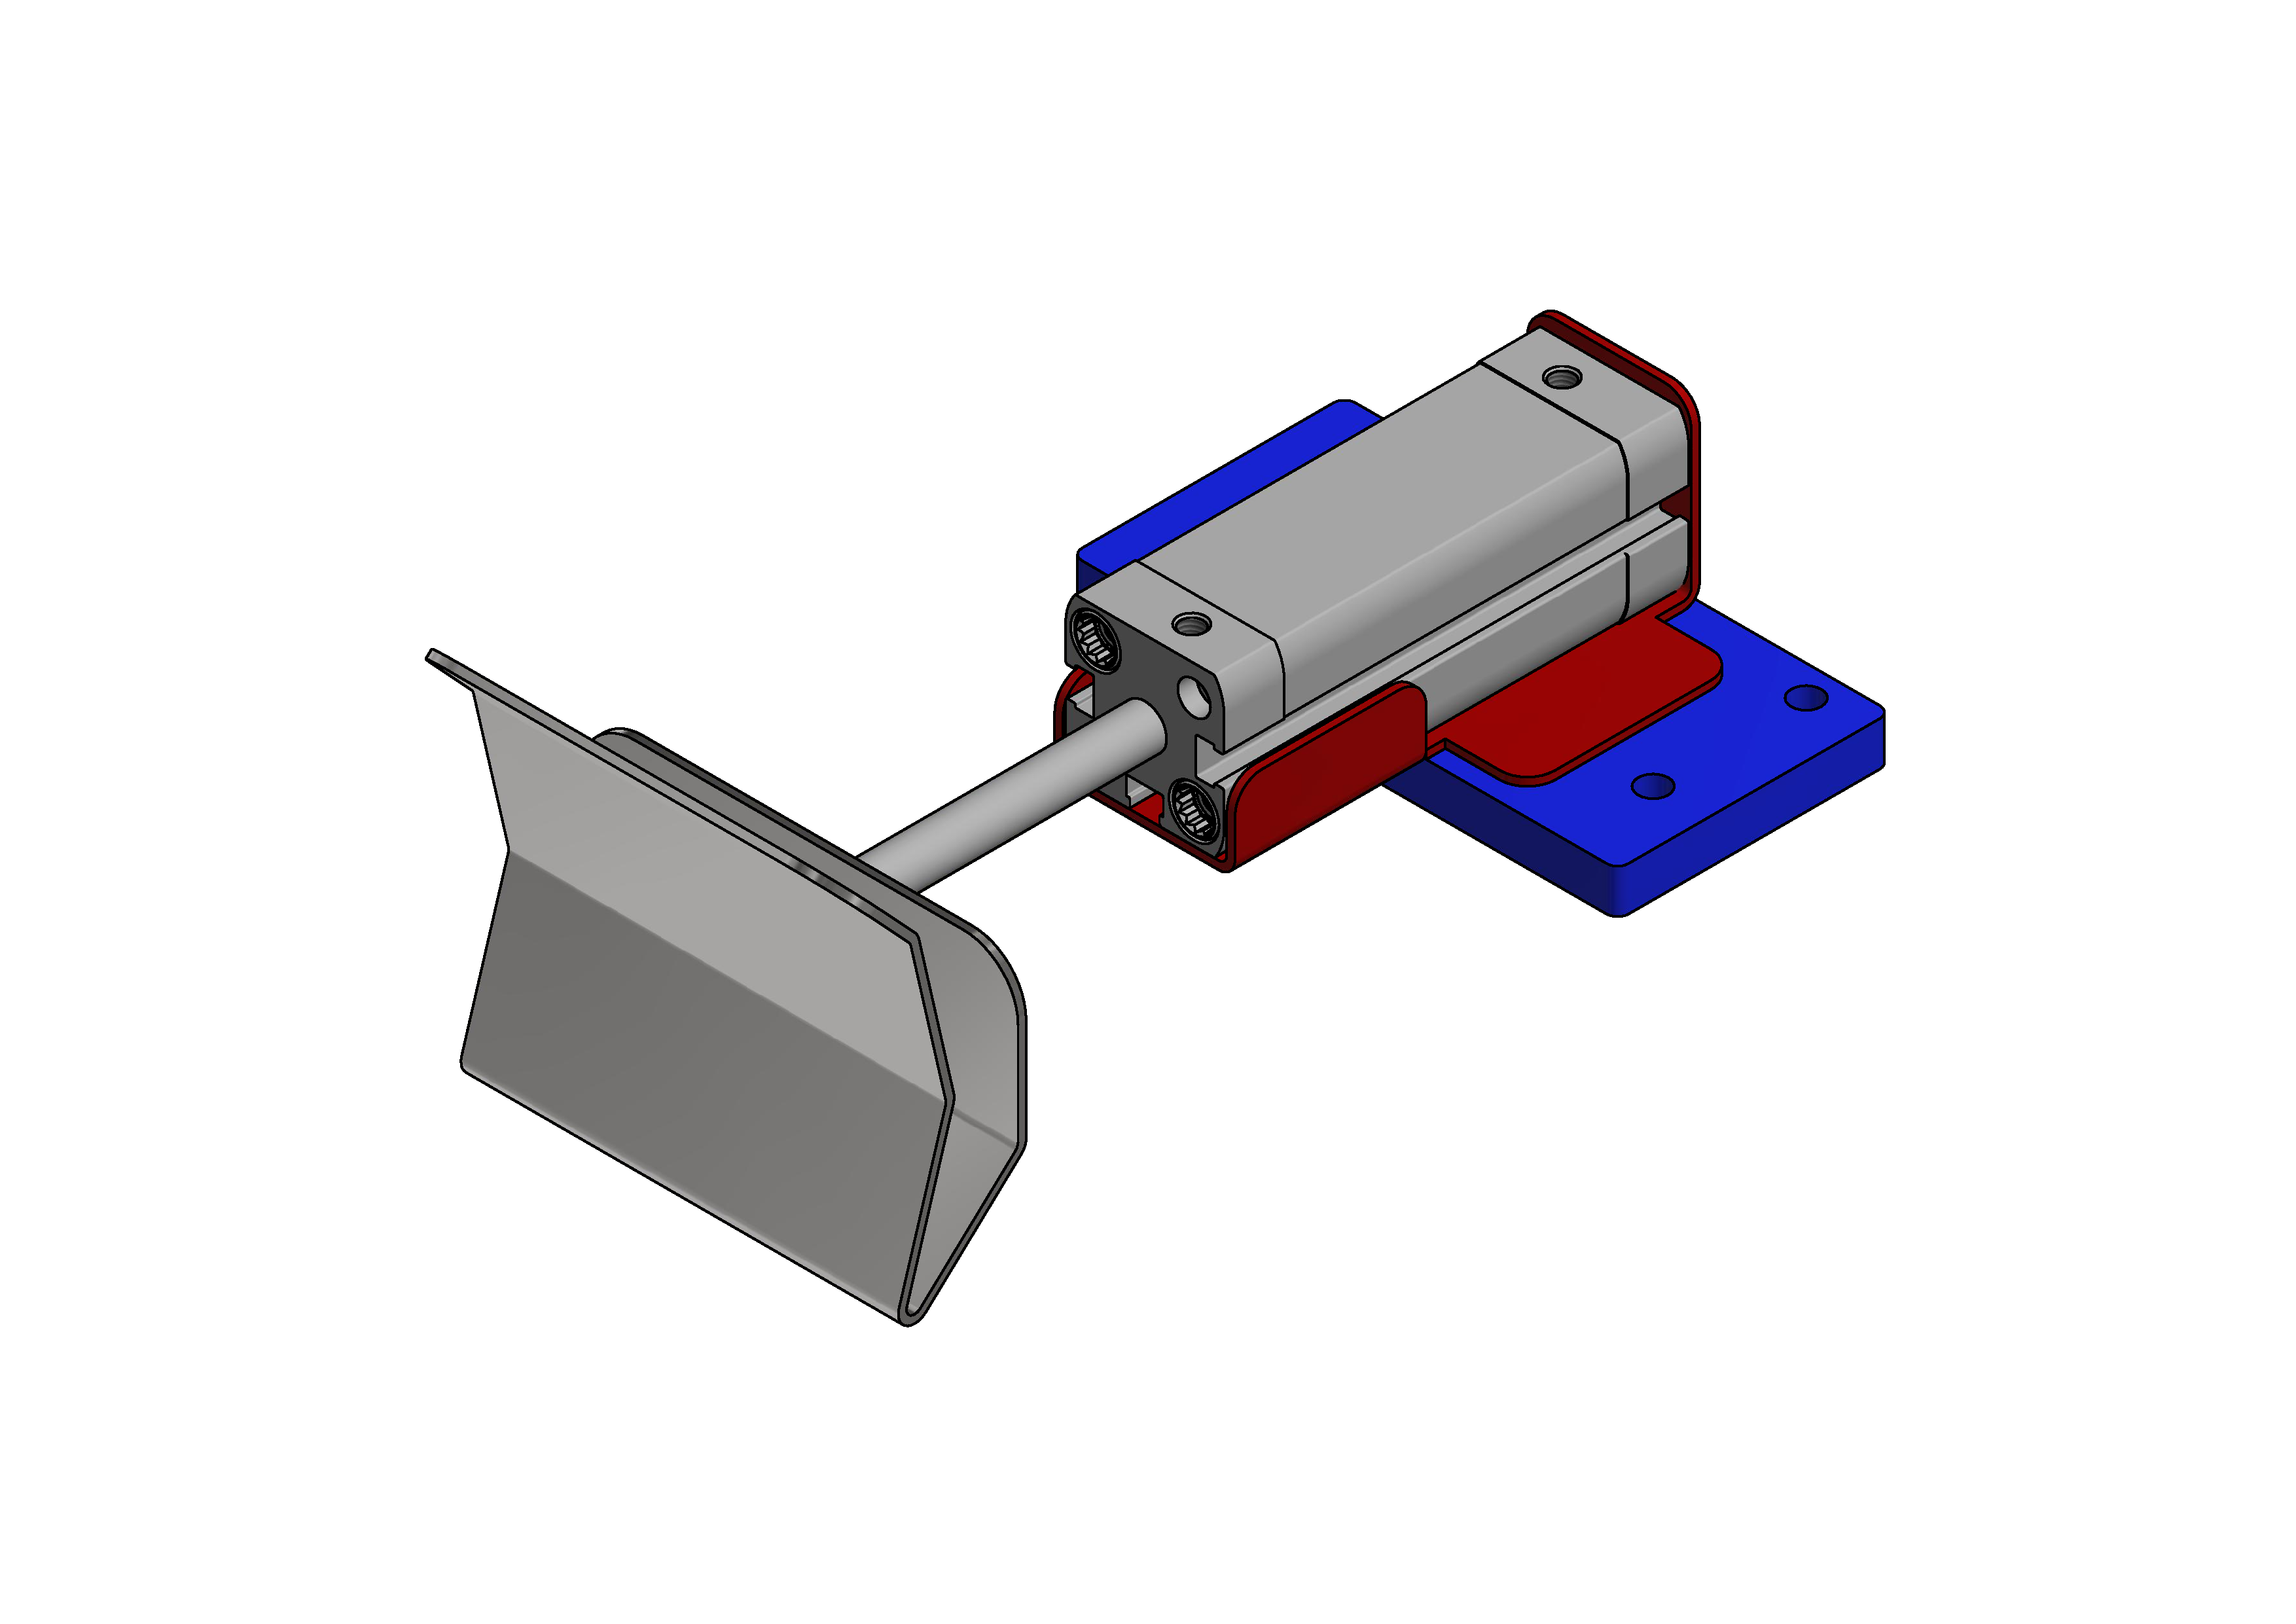
\includegraphics[width=0.7\textwidth]{src/img/pinza.pdf}
  \caption{Pistone bloccaggio}
  \label{fig:pinzaggio}
\end{figure}
All’estremità del telaio sono presenti delle lamiere che garantiscono il corretto ingresso ed uscita del tubo dalla parte di trasporto e dei sensori per controllare la posizione di quest’ultimo. Il telaio è stato realizzato mediante l’uso di tubolari quadrati in acciaio, dove sono stati fissati i supporti per le parti nominate in precedenza.

\subsection{Taglio ed espulsione}
\begin{figure}[H]
  \centering
  \begin{subfigure}[H]{0.45\textwidth}
    \centering
    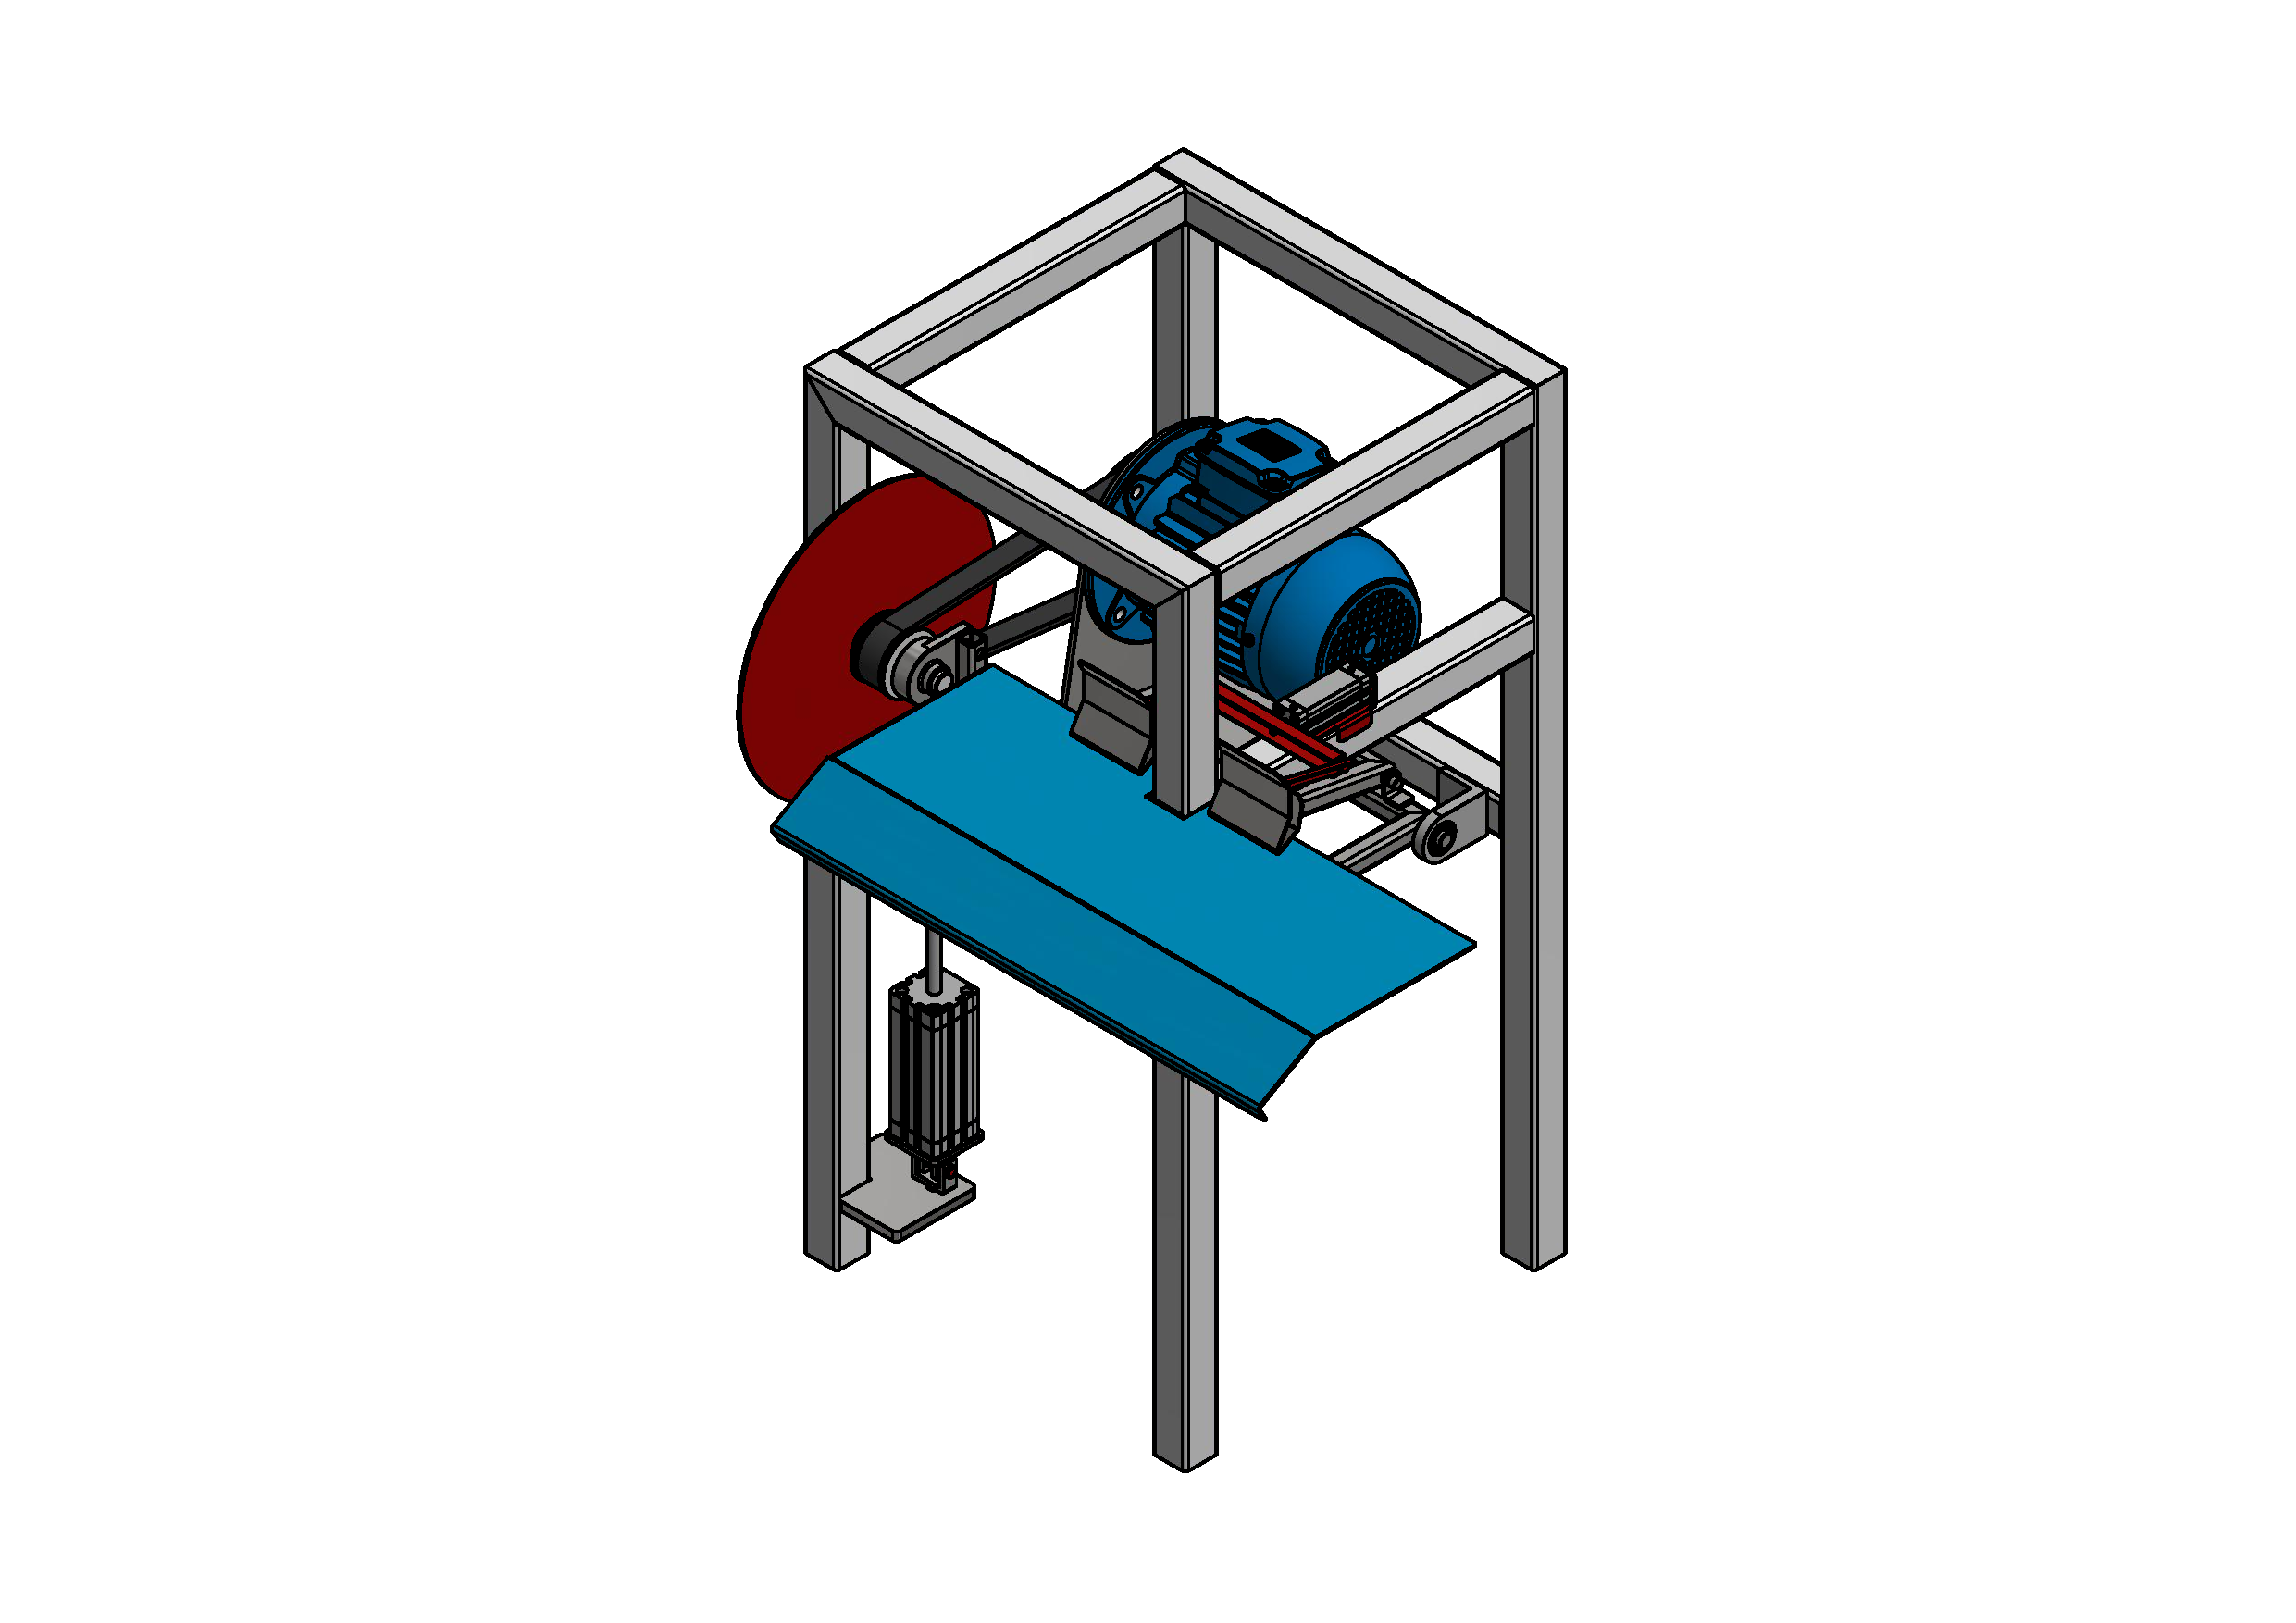
\includegraphics[width=\textwidth]{src/img/taglio_1.pdf}
  \end{subfigure}
  \hfill
  \begin{subfigure}[H]{0.45\textwidth}
    \centering
    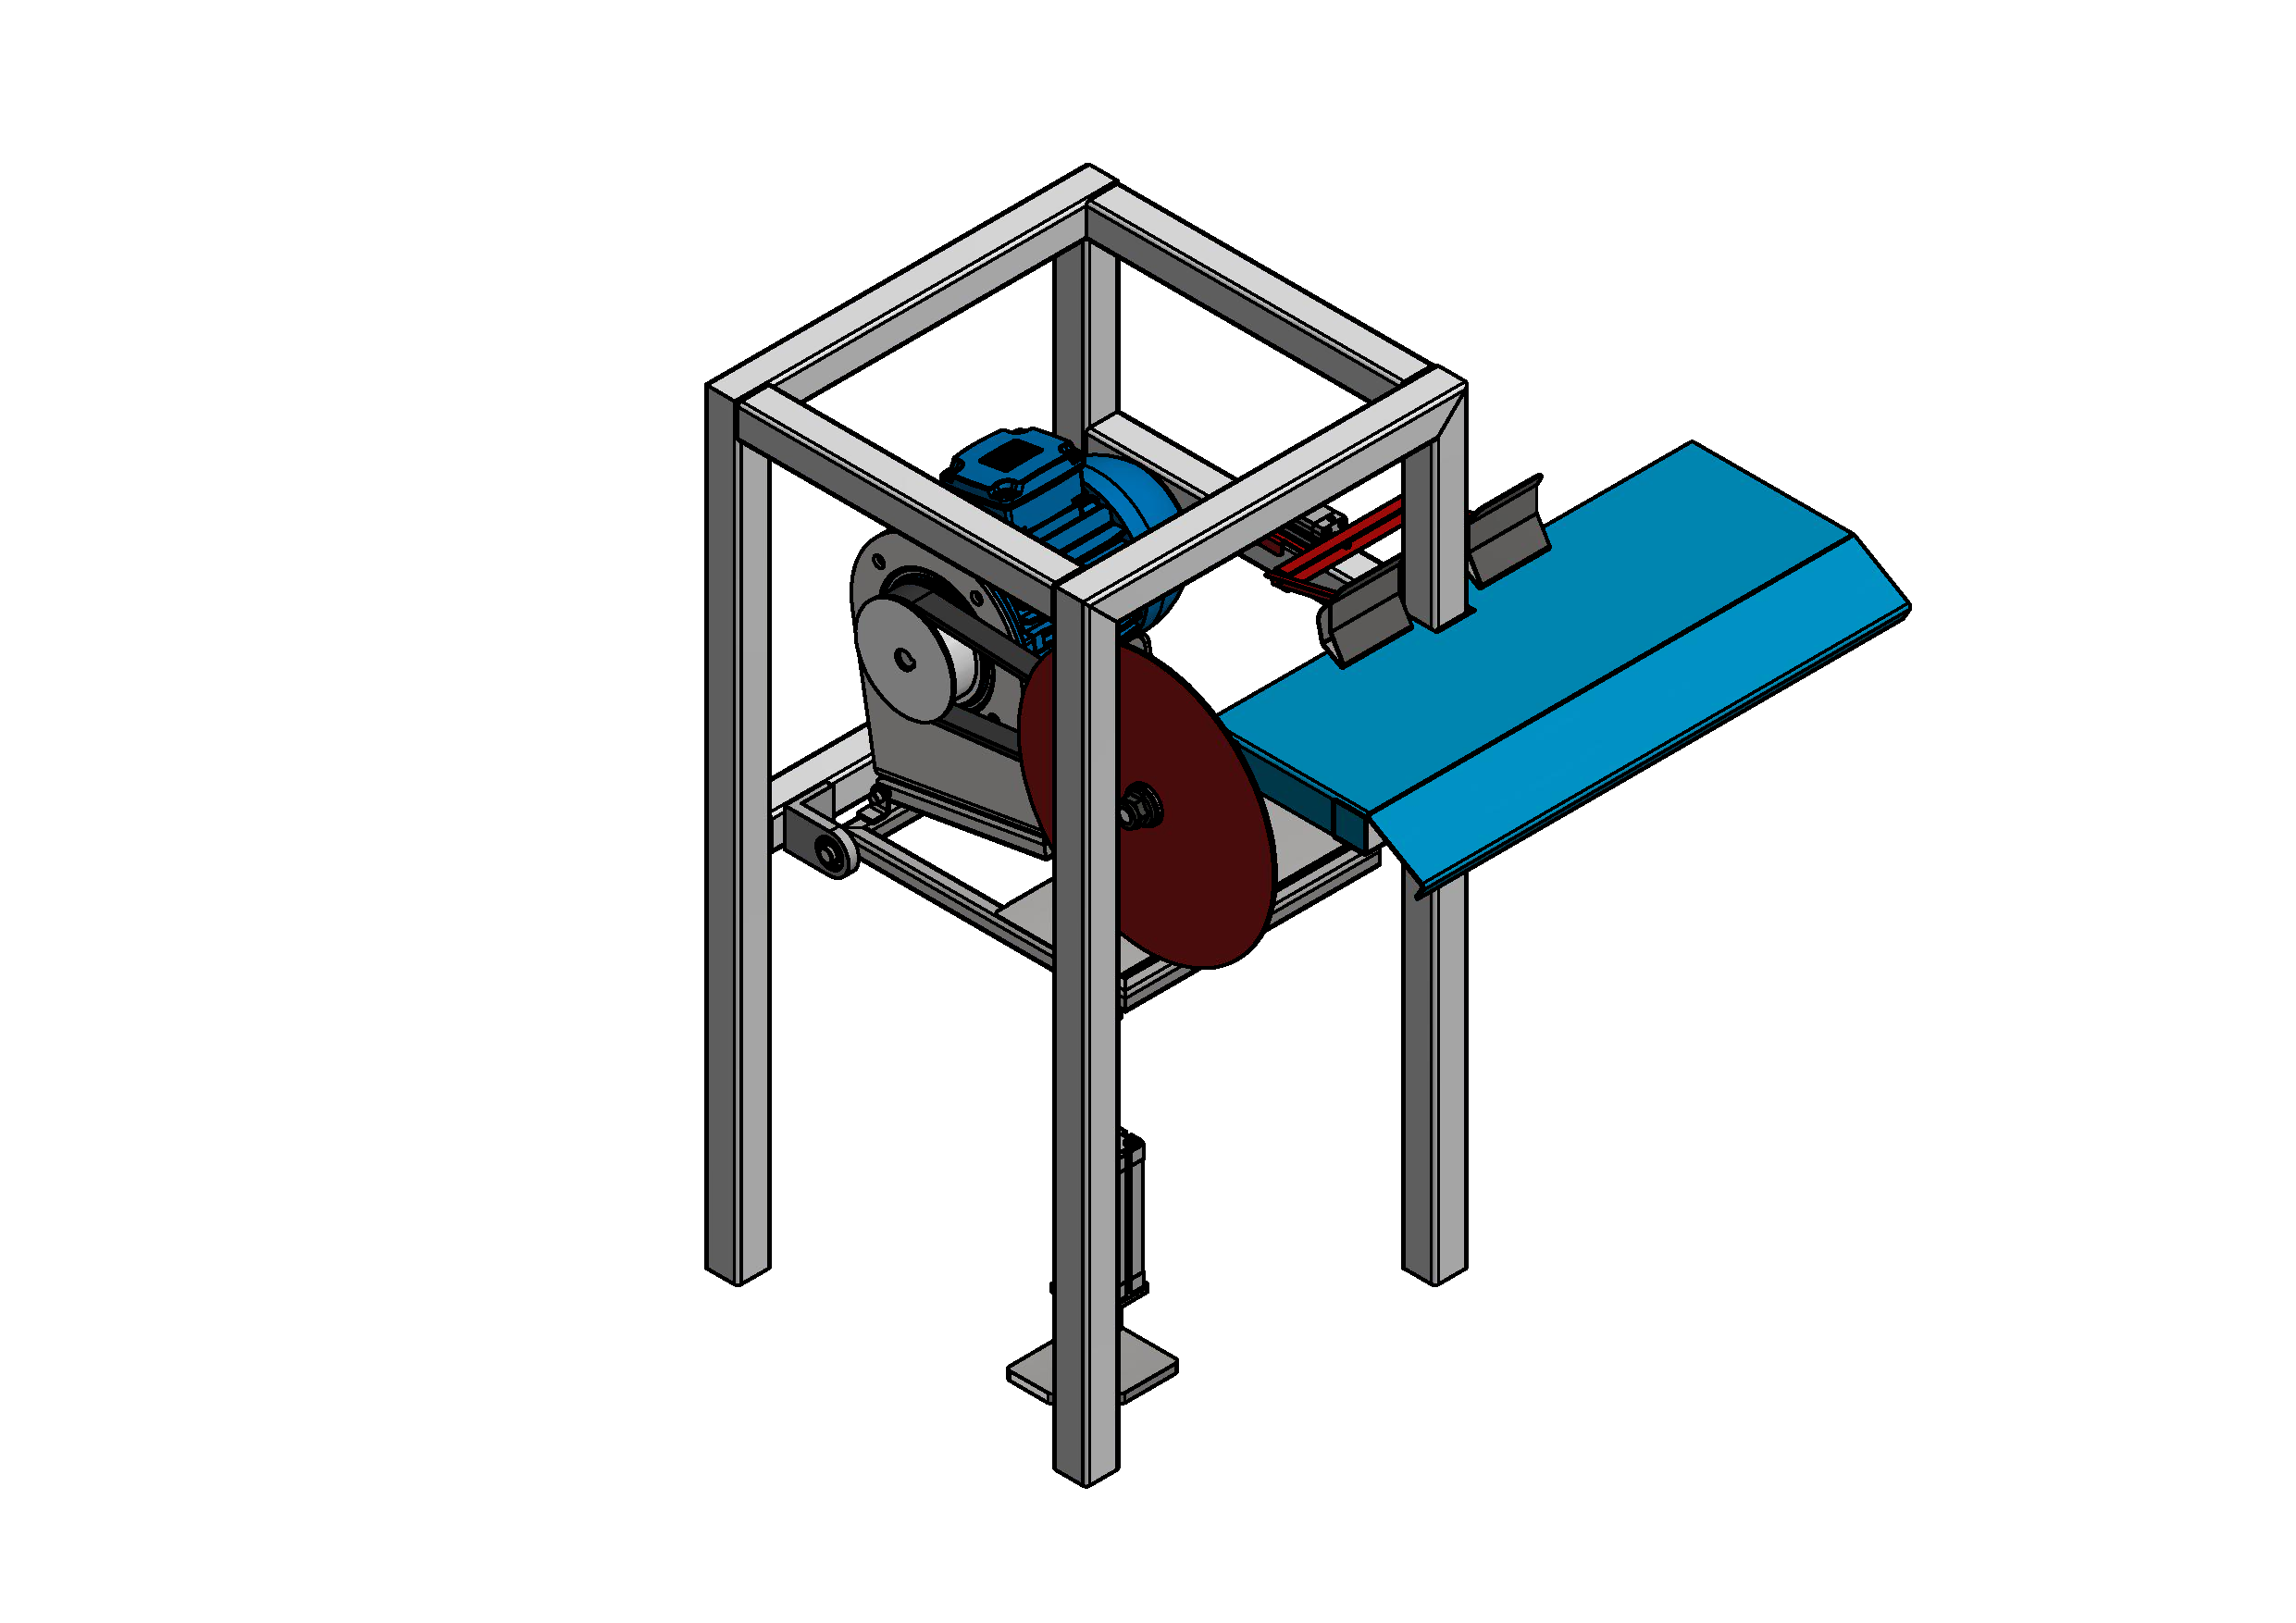
\includegraphics[width=\textwidth]{src/img/taglio_2.pdf}
    \end{subfigure}
    \caption{Gruppo taglio}
    \label{fig:vtcons}
\end{figure}
La seconda parte si occupa del taglio e l’espulsione del tubo mediante l’uso di una sega circolare ($D=\SI{300}{\mm}$) messa in moto da un motore elettrico monofase ($P = \SI{1,5}{\kW}$, $n_{max}=\SI{2500}{\rpm}$), il tutto collegato con una trasmissione a cinghie piatte con rapporto di trasmissione $i=\num{0.5}$ che si occupa di moltiplicare i giri della puleggia operatrice per garantire un taglio ottimale, come consigliato da tabella. Il sotto-assieme descritto è stato assemblato con un “telaietto” creato con dei tubolari quadrati in acciaio di piccole dimensioni per contenere il peso complessivo (motore, trasmissione, porta cuscinetto e lama) e vincolato ad un’estremità con 2 perni (che generano un effetto cerniera) che permettono la salita e la discesa di quest’ultimo mediante un pistone a doppio effetto (3MX). Per trasformare lo spostamento lineare del pistone in angolare dovuto alla rotazione attorno ai perni sono stati montati dei perni a forcella, collocati tra una piastra fissa e la base del pistone e tra l’estremità dello stelo e il telaietto, garantendo una buona spinta senza considerevoli perdite di forze. 

Infine, troviamo l’espulsione del pezzo lavorato grazie all’utilizzo di un pistone pneumatico (4M1) dove all’estremità dello stelo è stata fissata una lamiera con delle prolunghe laterali che fanno scorrere il tubo su un piano d’appoggio (con la possibilità di essere allungato in base alla lunghezza del tubo desiderata) verso una caduta libera.
\begin{figure}[H]
  \centering
  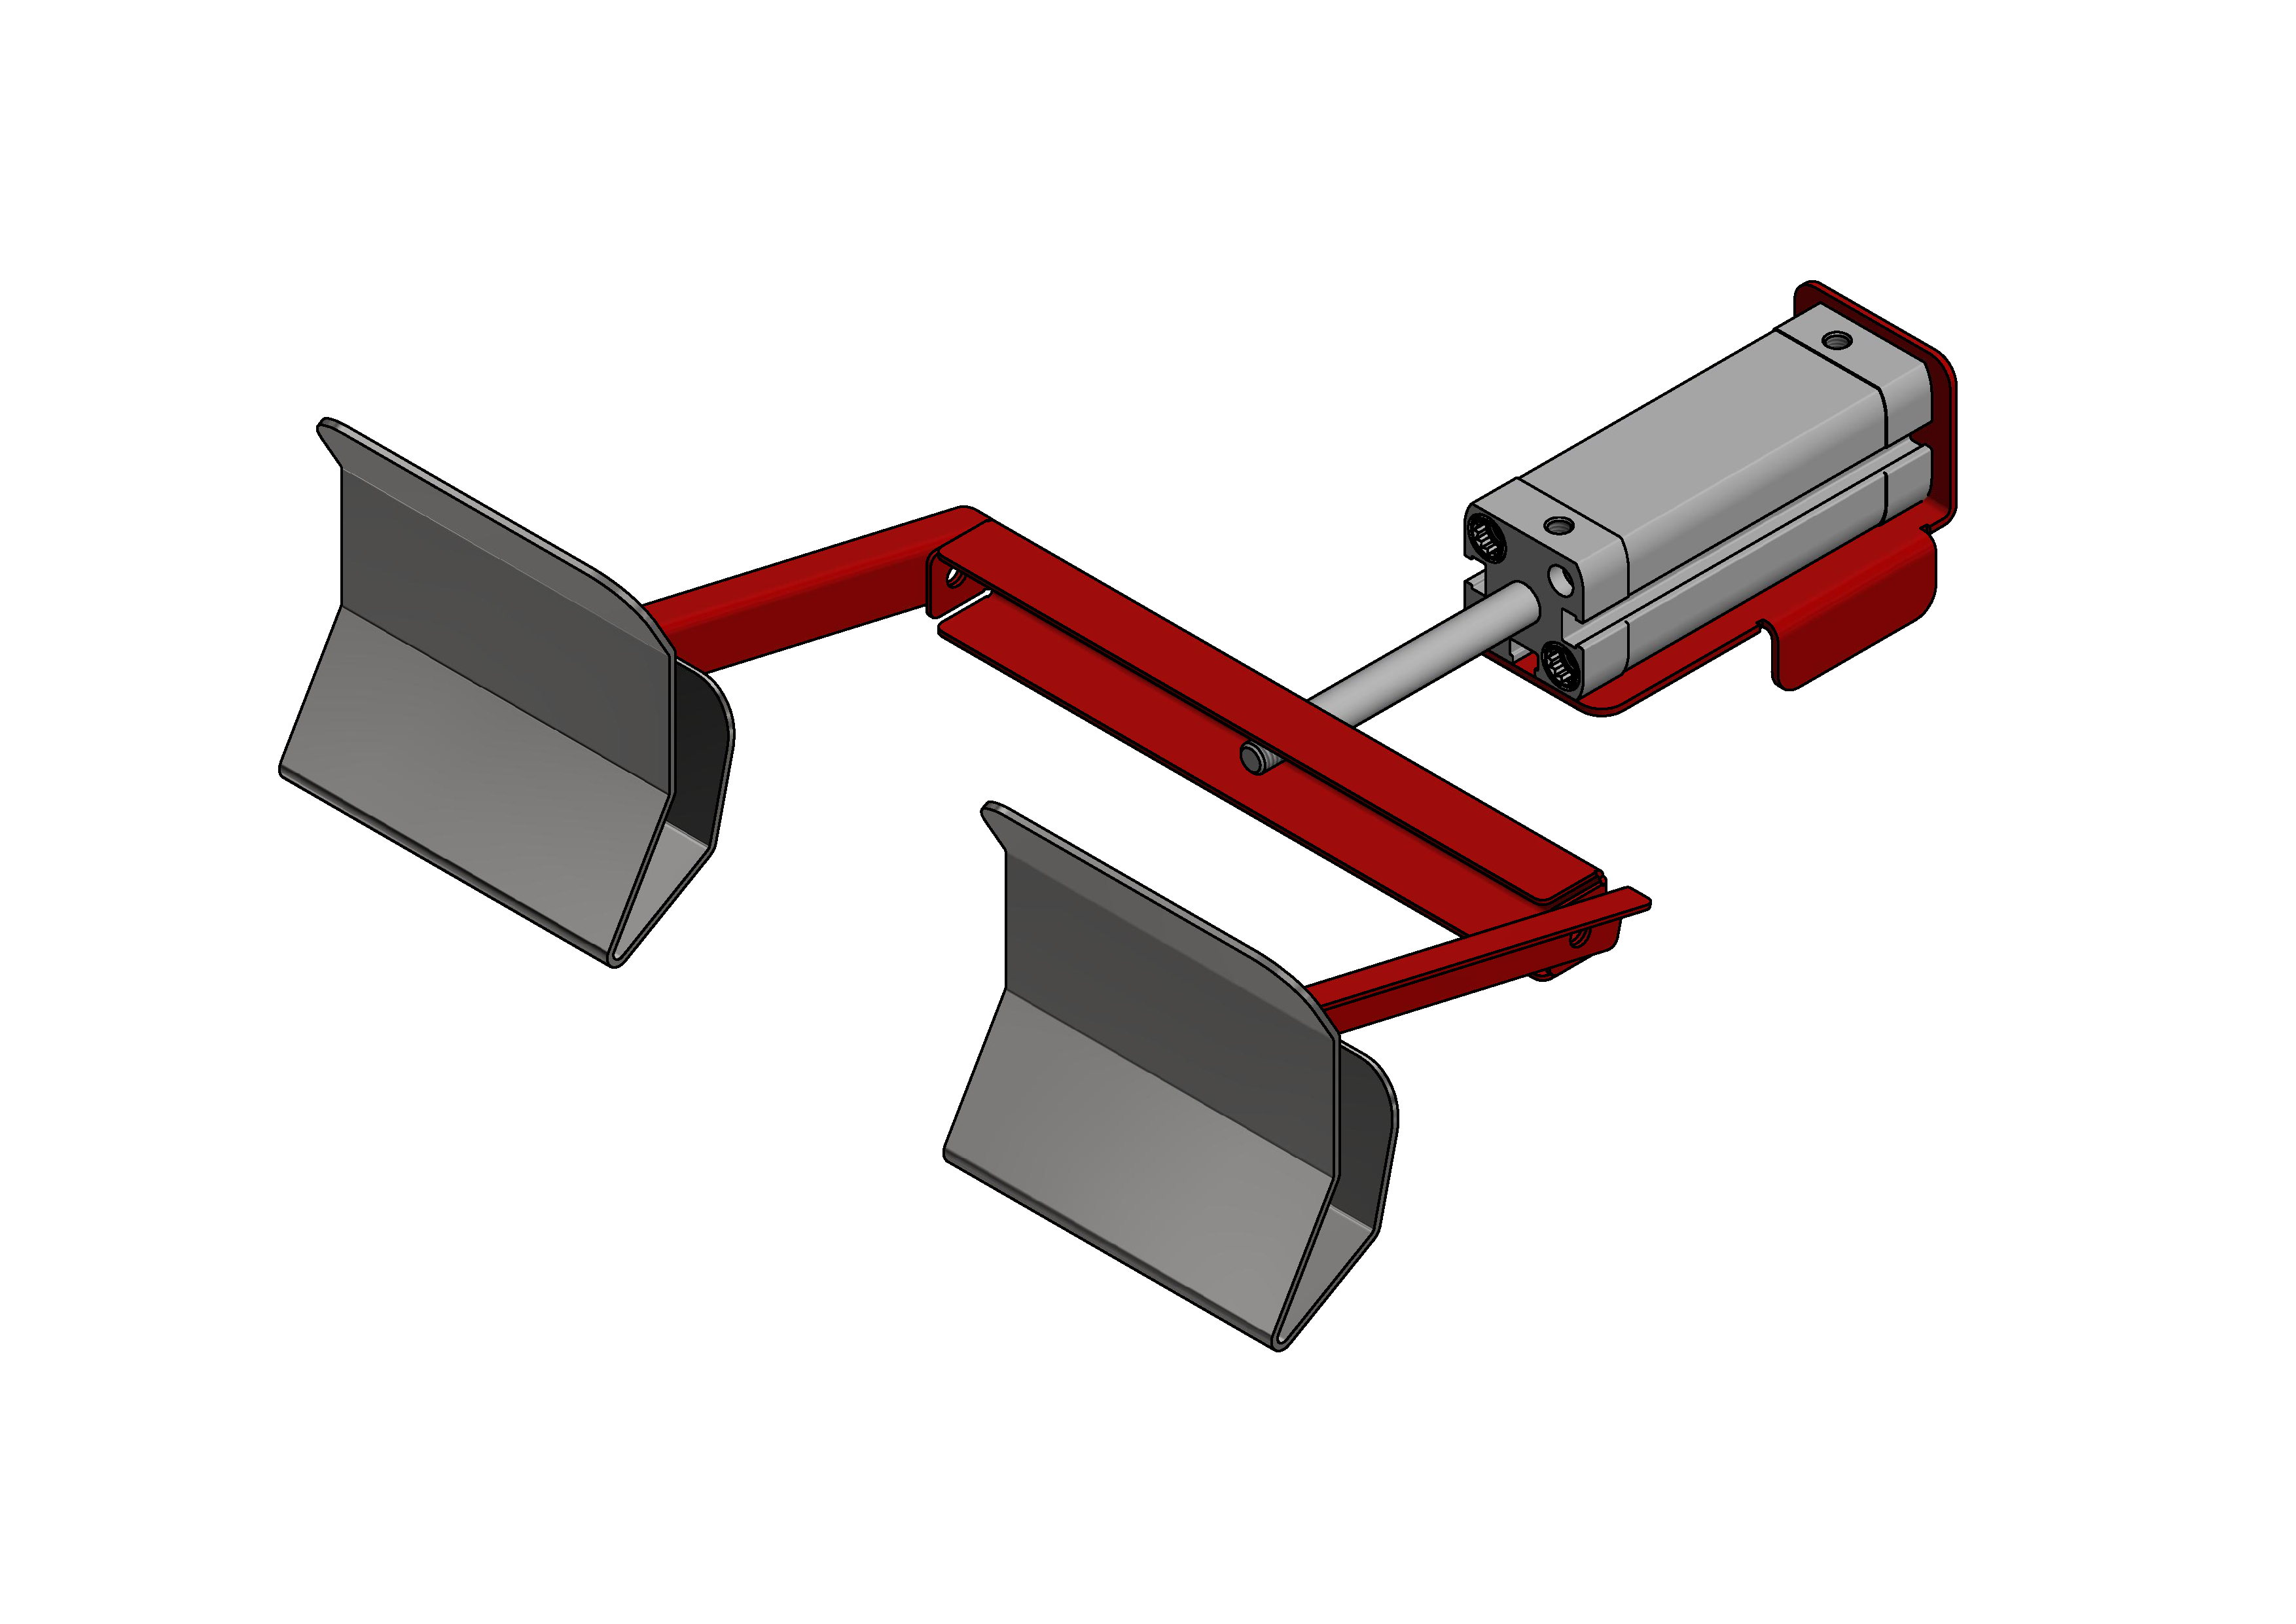
\includegraphics[width=0.7\textwidth]{src/img/espulsione.pdf}
  \caption{Pistone espulsione}
  \label{fig:espulsione}
\end{figure}
Il telaio portante è stato realizzato mediante l’uso di tubolari quadrati in acciaio, dove sono stati fissati i supporti per le parti nominate in precedenza.

\section{Calcoli di progetto}
\subsection{Calcolo dei giri utili del motore}
I tubi da tagliare, utilizzati per il trasporto di fluidi possono esseri creati con 3 diversi materiali plastici:
\begin{itemize}
\item PVC (cloruro di polivinile) con	$R_m = \SI{55}{\MPa}$;
\item PVC-C $R_m = \SI{60}{\MPa}$;
\item PE (polietilene) $R_m = \SI{17}{\MPa}$;
\item PP (polipropilene) $R_m = \SI{35}{\MPa}$.
\end{itemize}
PVC, PE e PP fanno parte della famiglia dei pannelli termoplastici (tabella $V_t$ consigliate) dove la velocità di taglio $V_t$ consigliata si aggira tra $\SIrange{50}{75}{\m\per\s}$ e l’avanzamento tra $\SIrange{0.05}{0.1}{\mm\per\s}$.

\begin{figure}[H]
    \centering
    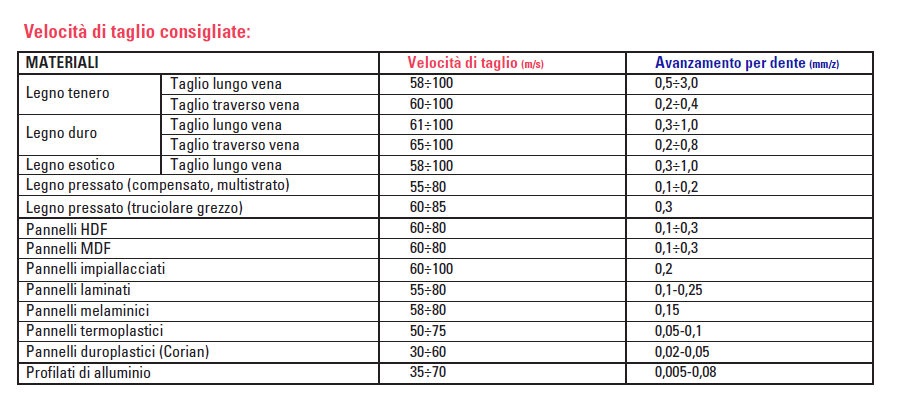
\includegraphics[width = 1\textwidth]{src/img/Vtaglio_lama.png}
    \caption{$V_t$ consigliate}
    \label{fig:vtcons}
\end{figure}

Seguendo la linea nera (per materiali plastici) della tabella, si assume un diametro della lama circolare di $D=\SI{300}{\mm}$ (inoltre utilizzata nella maggior parte dei casi, grazie al suo ottimo rapporto efficienza/ingombro).

\begin{figure}[H]
    \centering
    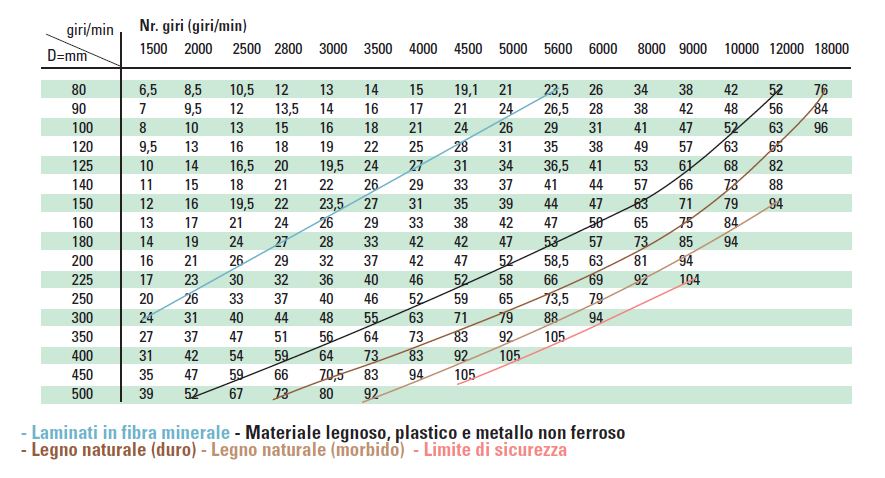
\includegraphics[width = 1\textwidth]{src/img/Vtaglio_lama_grafico.png}
    \caption{Grafico $V_t$ consigliate}
    \label{fig:grafvtcons}
\end{figure}

Conoscendo la $V_t$ richiesta dal materiale per essere tagliato possiamo calcolare il numero di giri generati dal motore, che successivamente verranno moltiplicati mediante una trasmissione a cinghie piatte.
Sapendo che:
\begin{equation}
  \omega=\frac{V_t}{r_{lama}}
\end{equation}
Si calcola:
\begin{itemize}
\item $\omega_{min} = \frac{V_t}{r} = \frac{\SI{50}{\m\per\s}}{\SI{0,15}{\m}} = \SI{334}{\radian\per\s} $;
\item $\omega_{max}  = \frac{V_t}{r}= \frac{75}{0,15} = \SI{500}{\radian\per\s}$.
\end{itemize}

Per una lettura più comoda si converte la $\omega$ in rpm mediante la seguente formula:
\begin{equation}
  n = \frac{60\omega}{2\pi}
\end{equation}

Quindi:
\begin{description}
\item $n_{min} = \frac{334\cdot 60}{2\pi} \approx \SI{3200}{\rpm}$;
\item $n_{max} = \frac{500\cdot 60}{2\pi} \approx \SI{4800}{\rpm}$.
\end{description}

Conoscendo questi dati, con l’intenzione di utilizzare una trasmissione a cinghie piatte con un rapporto di trasmissione $i = \num{0,5}$ (che moltiplica la velocità della puleggia operatrice del doppio rispetto a quella motrice) si può restringere il campo di ricerca del motore monofase fino a \SI{2500}{\rpm} massimi che, grazie alla trasmissione, potrà raggiungere i \SI{5000}{\rpm}.

\subsection{Calcolo della forza di taglio}
La taglia del tubo da tagliare, nel nostro caso, ha le seguenti dimensioni:
\begin{description}
\item $D = \SI{104}{\mm}$
\item $d = \SI{100}{\mm}$
\item $A = \SI{641}{\mm\squared}$
\end{description}

Utilizzando il carico di rottura del materiale più resistente (PVC-C) con $\sigma = \SI{60}{\MPa}$, si calcola la sua $\tau$, sapendo che $\tau = \frac{\sigma}{\sqrt{3}}$ e di conseguenza $\tau = k\frac{F}{A}$ dove per sezioni circolari $k=4/3$. Rovesciando la formula si può calcolare la $F$ necessaria per tagliare il tubo:

\begin{equation}
\tau=\frac{60}{\sqrt{3}} = \SI{35}{\MPa}
\end{equation}
\begin{equation}
F = \frac{A\tau}{k} = \SI{16,7}{\kN}
\end{equation}

\subsection{Calcolo della potenza del motore}
Per il calcolo della potenza del motore, dopo aver trovato il numero di giri necessari, è stato utilizzato il metodo sperimentale. Grazie alla presenza di una sega circolare (da falegnameria) e il tubo da lavorare, dopo varie prove e tagli siamo giunti alla conclusione di adottare un motore con una potenza di \SI{1,5}{\kW}. La possibilità di provare il taglio ci ha permesso di stabilire le seguenti considerazioni:
\begin{itemize}
\item Le velocità di taglio, calcolate in precedenza sono state del tutto coerenti con le prove effettuate.
\item La velocità di avanzamento, invece, ha soddisfatto le aspettative con un andamento lento e costante, senza imprimere troppa forza (circa \SI{50}{\N}) tra il tubo e la lama per evitare che quest'ultima si bloccasse.
  \end{itemize}
  \subsection{Dimensionamento della trasmissione}
  \begin{figure}[H]
    \centering
    \begin{subfigure}[H]{0.45\textwidth}
    \centering
    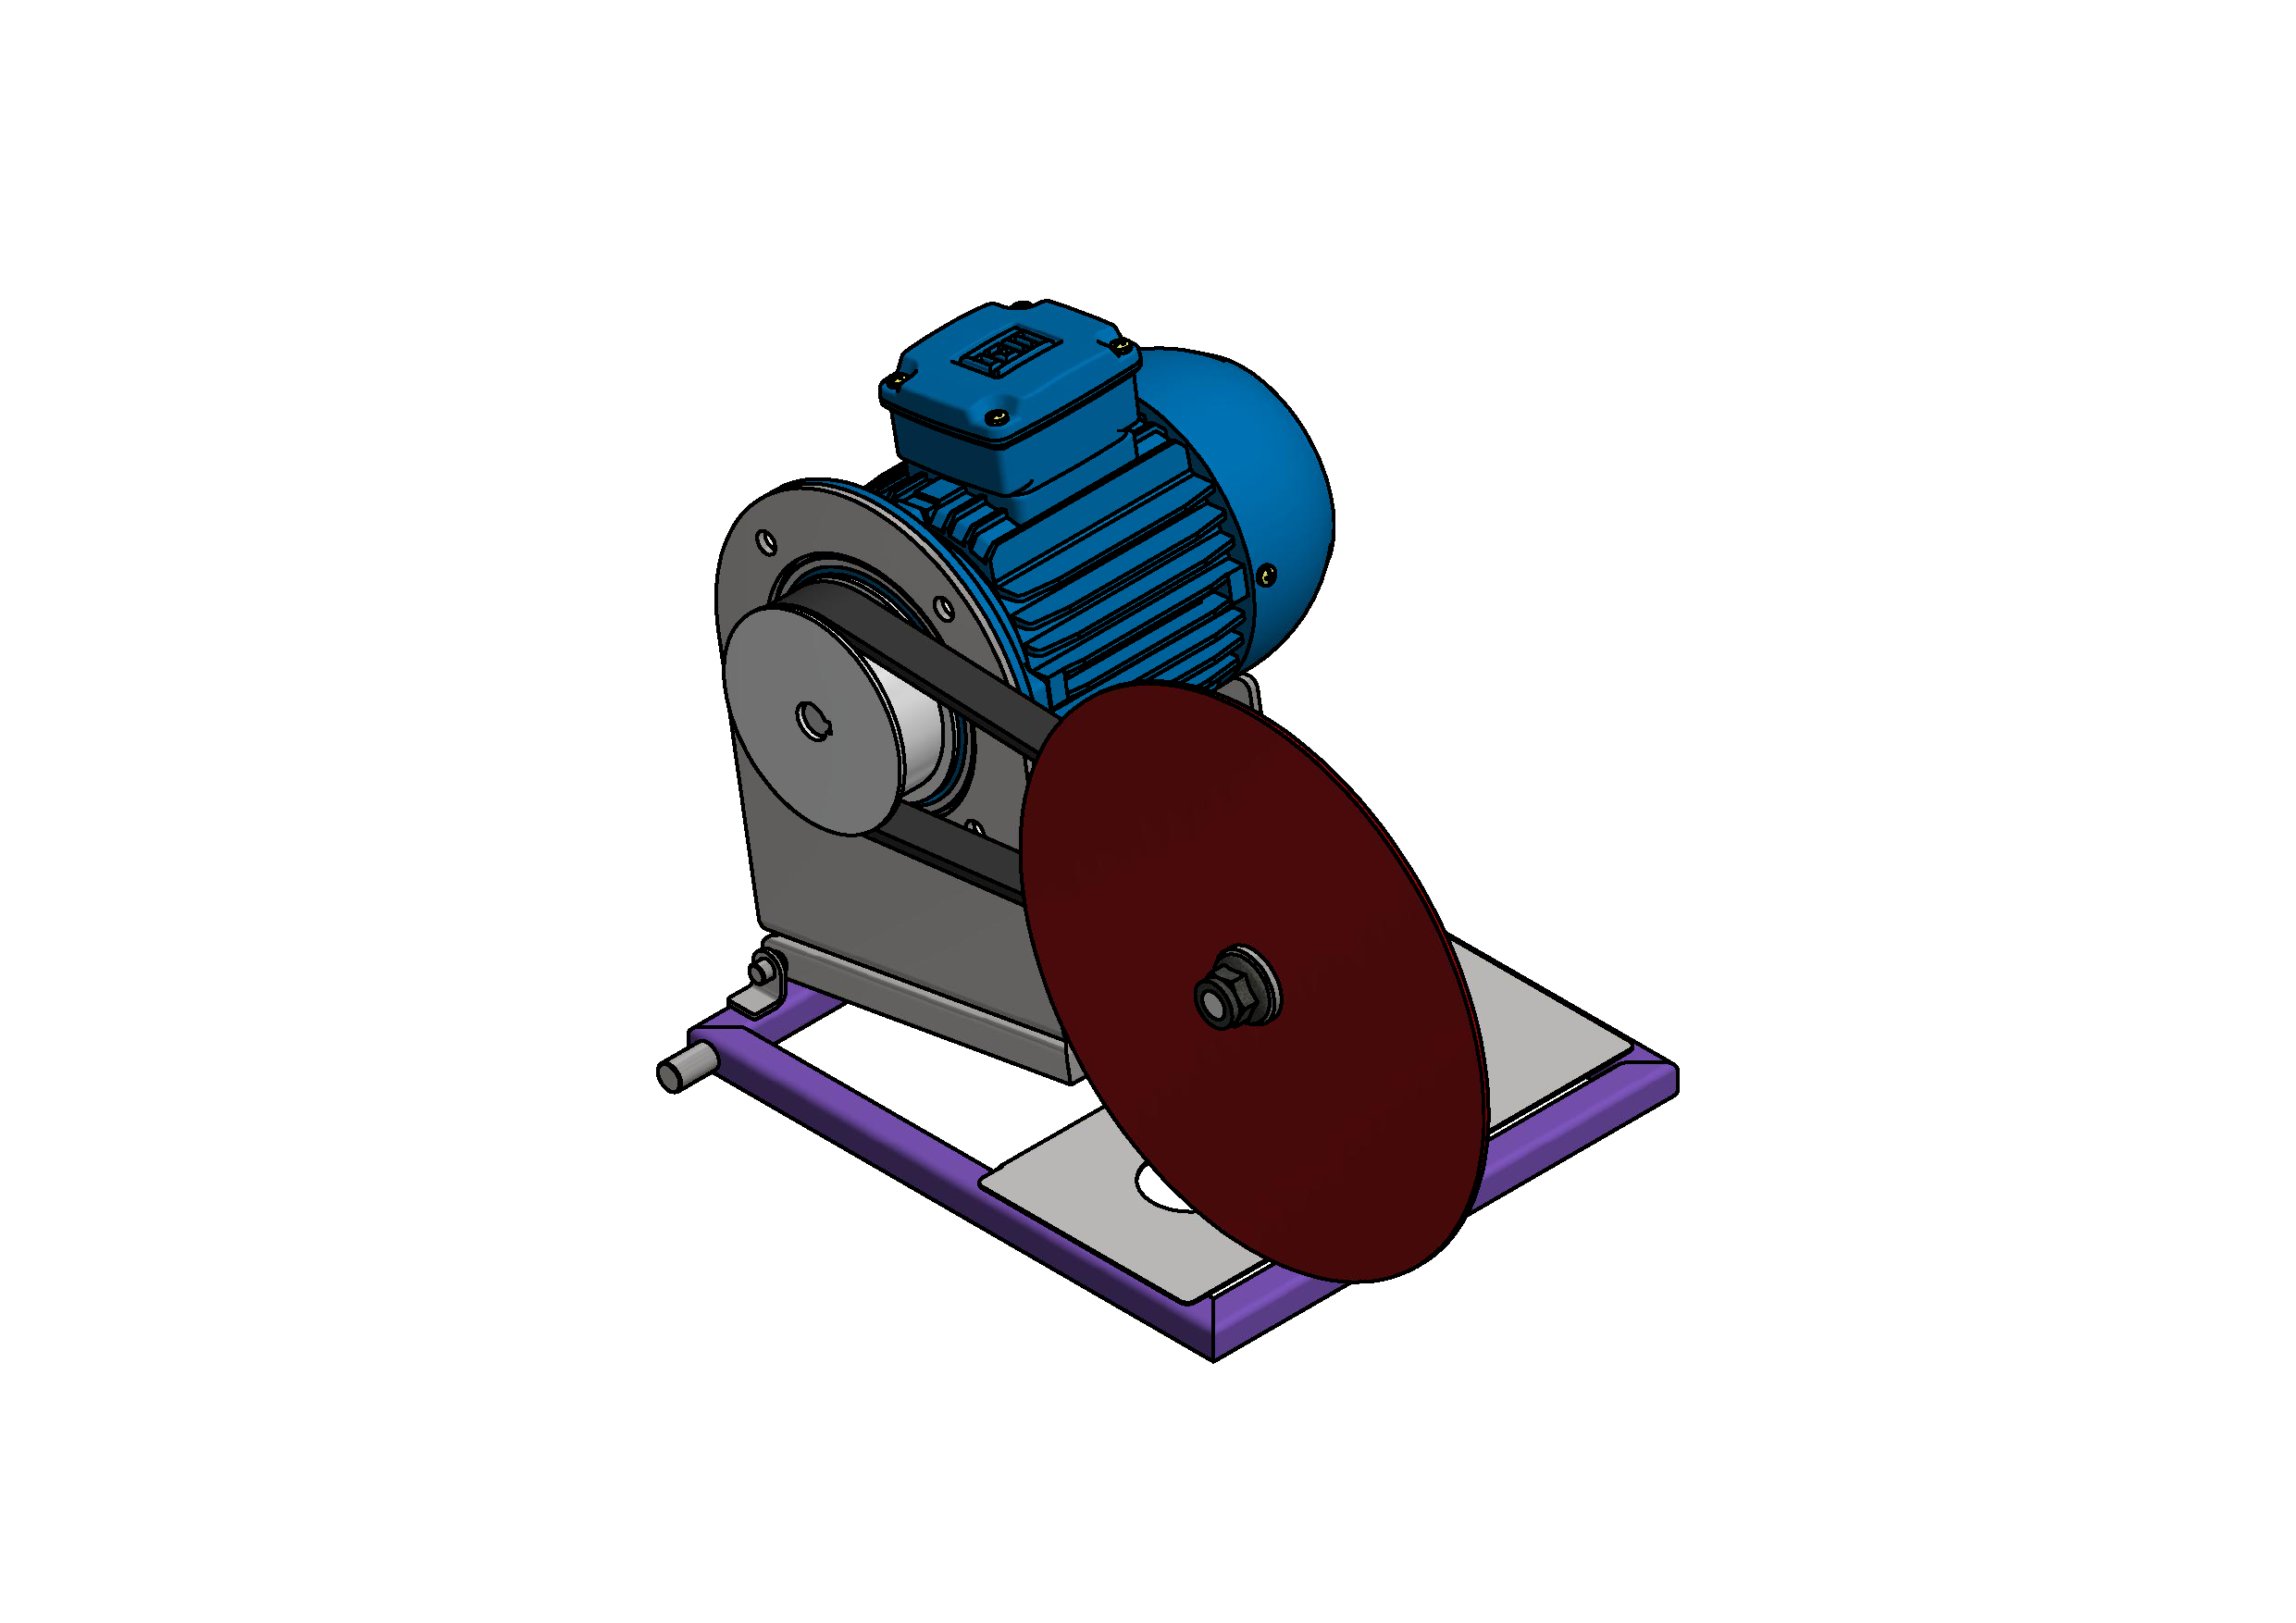
\includegraphics[width=\textwidth]{src/img/sega_1.pdf}
  \end{subfigure}
  \hfill
  \begin{subfigure}[H]{0.45\textwidth}
    \centering
    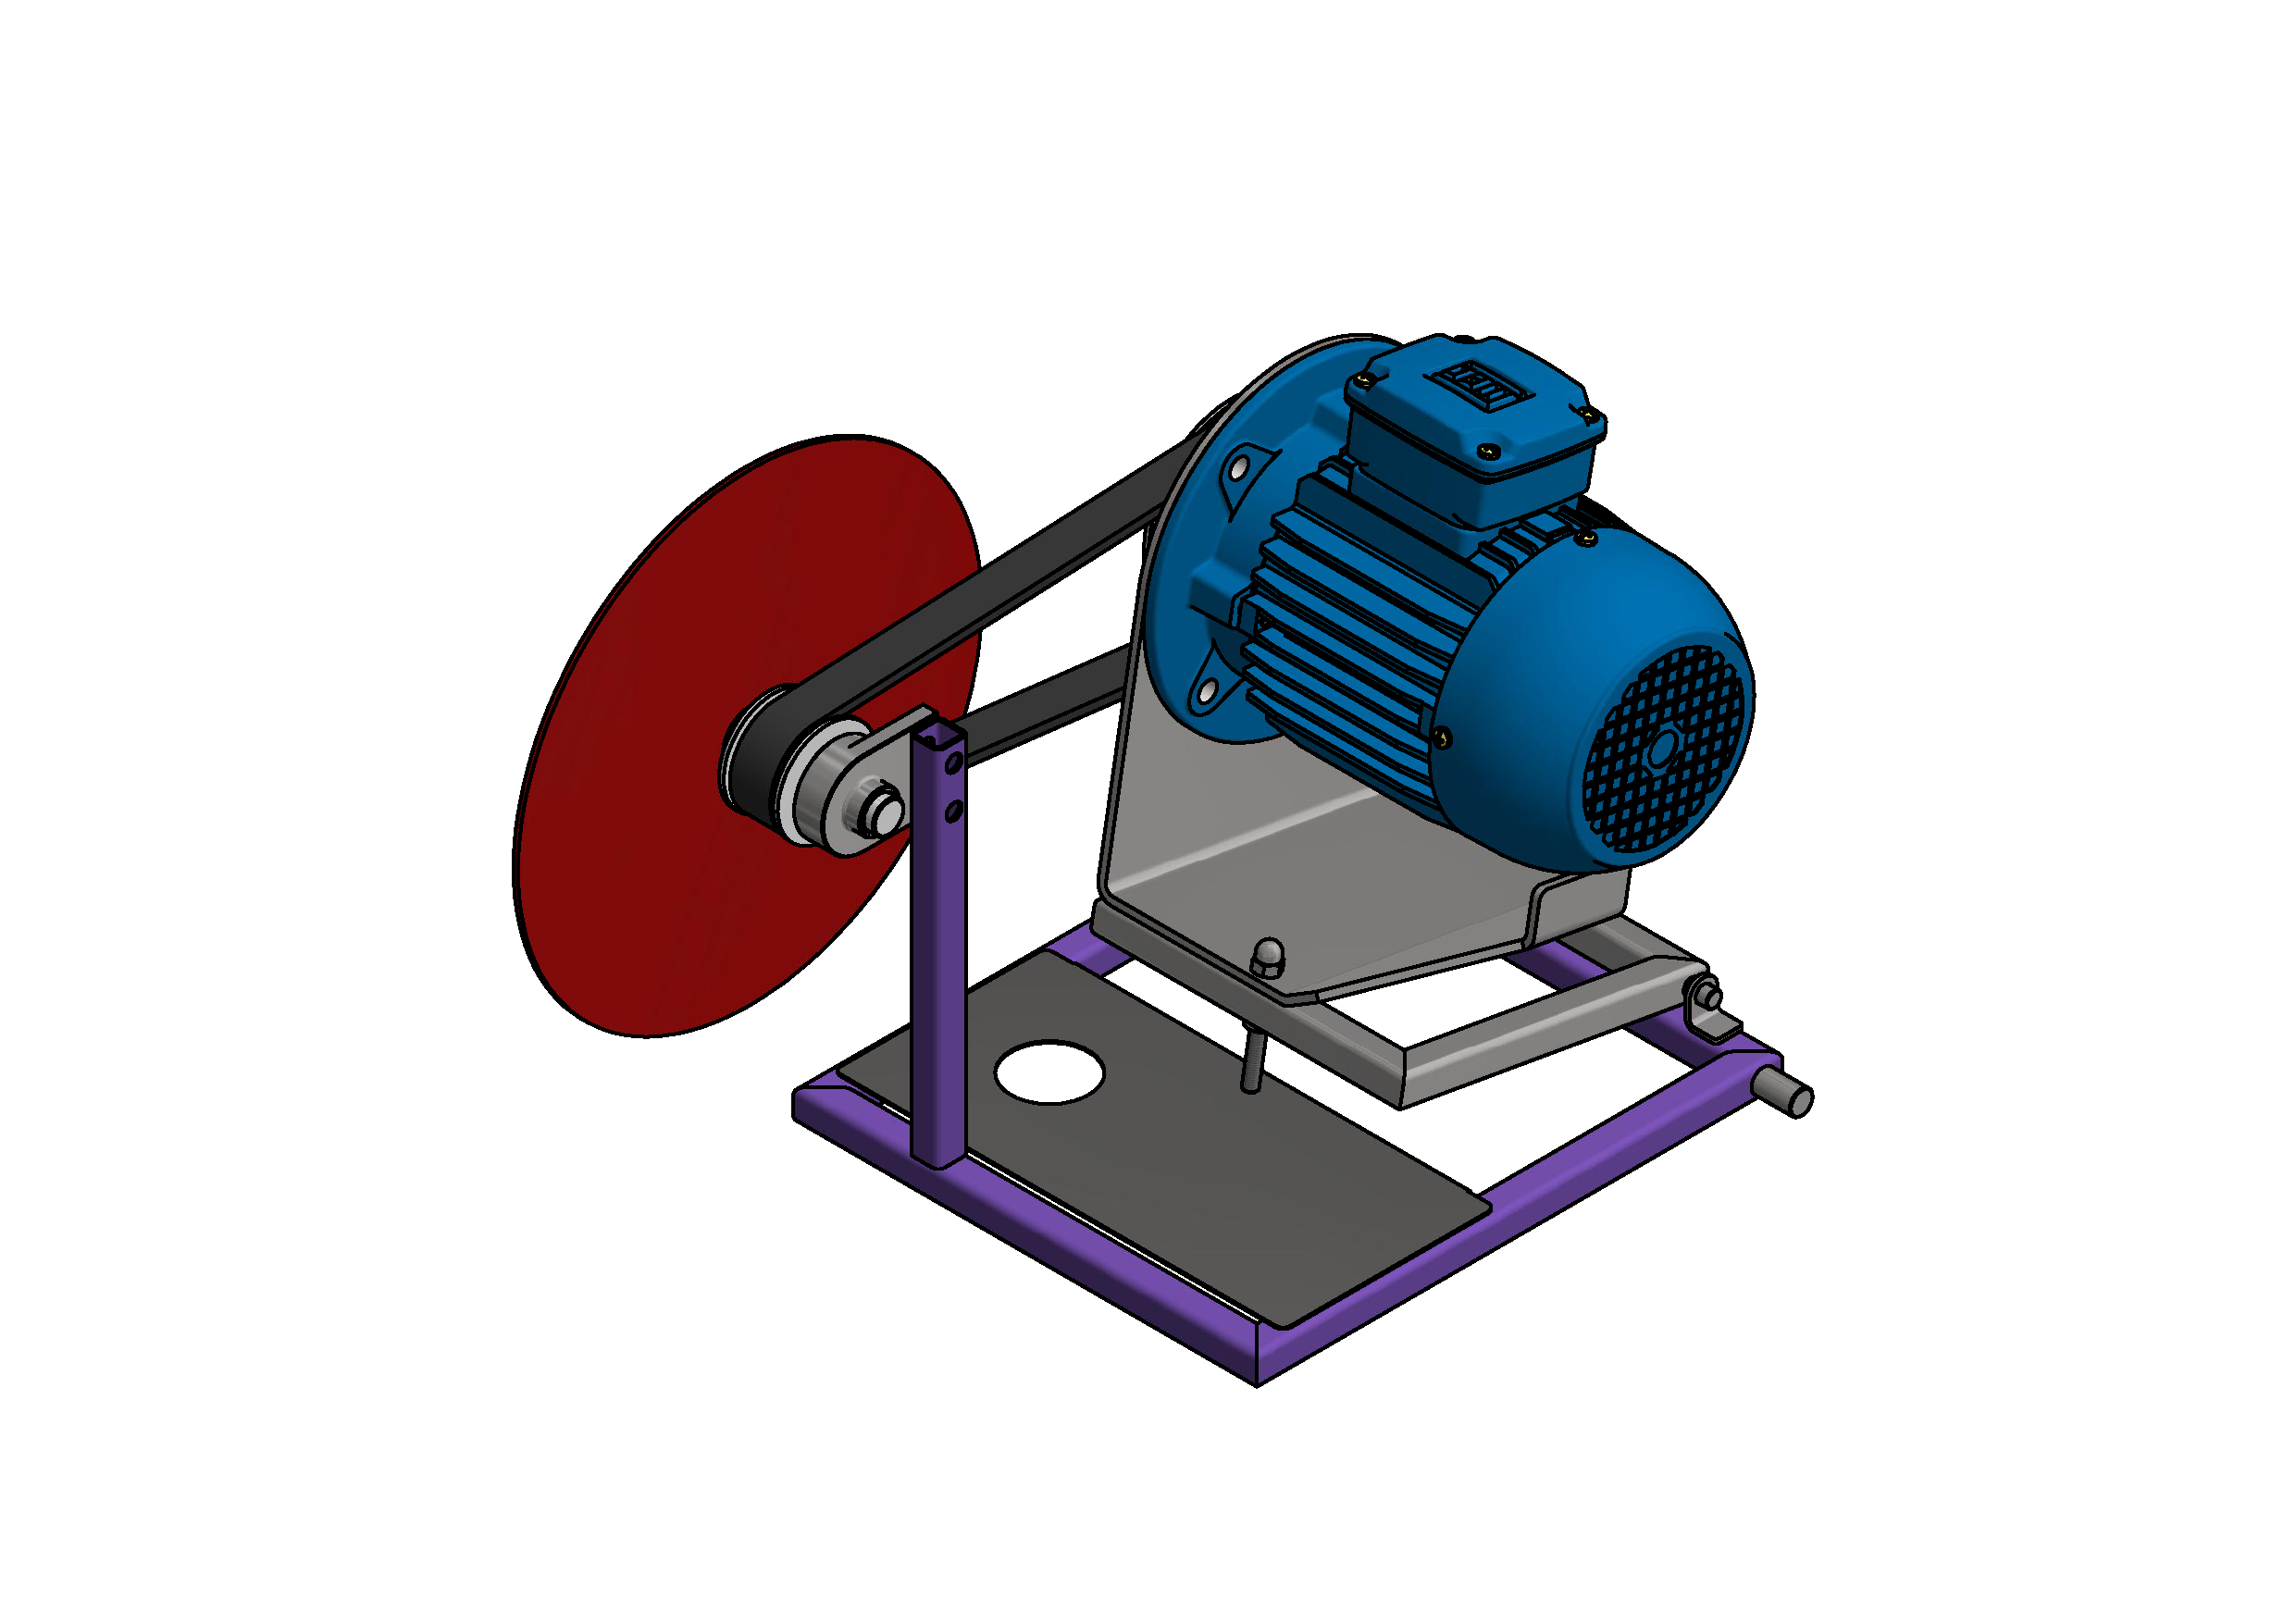
\includegraphics[width=\textwidth]{src/img/sega_2.pdf}
    \end{subfigure}
    \caption{Gruppo trasmissione}
    \label{fig:vtcons}
\end{figure}
Le cinghie sono organi flessibili impiegati nella trasmissione di potenza da una puleggia motrice a una condotta, montate su alberi disposti ad una certa distanza (interasse). Le cinghie possono appartenere a due gruppi distinti: cinghie di tipo convenzionale e cinghie sincrone.
Le cinghie di tipo convenzionale trasmettono il moto sfruttando l’aderenza (attrito) con il profilo esterno della puleggia. In questo caso possono verificarsi scorrimenti fra la cinghia e la puleggia durante il moto.
Le cinghie sincrone trasmettono il moto tramite l’ingranamento dei denti della cinghia con quelli della puleggia. Non sono soggette a scorrimento e necessitano di un precarico molto modesto.
Industrialmente sono usate cinghie piatte, trapezoidali e sincrone.
Per dimensionare una trasmissione partiamo dai dati del motore, forniti dal datasheet:

\begin{table}[H]
\centering
\begin{tabular}{|l|c|}
\hline
\multicolumn{2}{|c|}{\textbf{Dati motore}} \\ \hline
Potenza & \SI{1,5}{\kW} \\ \hline
Giri motore & \SI{2500}{\rpm} \\ \hline
Diametro albero & \SI{19}{\mm} \\ \hline
\end{tabular}
\end{table}

Successivamente, una volta trovato il numero di giri che vogliamo sviluppare sull’operatrice ($n=\SI{5000}{\rpm}$), calcolo il rapporto di trasmissione ($i$) e l’interasse ($I$) tra i due elementi rotanti in base alla dimensione delle mie pulegge, che assumo a piacere dalla serie di Renard R20 a partire da un diametro minimo di \SI{40}{\mm}.

Assumiamo il diametro della puleggia motrice $D_m=\SI{100}{\mm}$ e di conseguenza (per rispettare il rapporto di trasmissione e la serie R20) $D_o=\SI{50}{\mm}$ per il diametro dell’operatrice. Questa scelta è giustificata dagli ingombri in fase di modellazione 3D per tagliare correttamente il tubo senza urti.
Il calcolo dell’interasse dipende dal carico, nel nostro caso $I\geq 3\cdot D_m$ per trasmissioni a carico variabile. Una volta rispettata questa condizione si può scegliere a piacimento la lunghezza in base alle esigenze (ingombri, etc...)

\begin{table}[H]
\centering
\resizebox{\textwidth}{!}{
\begin{tabular}{|l|c|l|}
\hline
\multicolumn{2}{|c|}{\textbf{Dati Pulegge}} & \multicolumn{1}{c|}{\textbf{Formula}} \\ \hline
Numero giri motrice ($n_m$) & \SI{2500}{\rpm} & Fornito dal motore \\ \hline
Numero giri operatrice ($n_o$) & \SI{5000}{\rpm} & $\frac{n_m}{i}$ \\ \hline
Rapporto di trasmissione ($i$) & \num{0,5} & $\frac{n_m}{n_o}$ \\ \hline
Diametro puleggia motrice ($D_m$) & \SI{100}{\mm} & Scelta personale rispettando R20 \\ \hline
Diametro puleggia operatrice ($D_o$) & \SI{50}{\mm} & $D_o=D_m\cdot i$ \\ \hline
Interasse ($I$) & \SI{300}{\mm} & $I=3\cdot D_m$ \\ \hline
\end{tabular}
}
\end{table}

Durante la progettazione di una trasmissione è importante consultare le tabelle unificate che forniscono dati di correzione in base ai materiali utilizzati per la realizzazione e il servizio che devono compiere.
Dati provenienti dalle tabelle del manuale di Meccanica:
\begin{table}[H]
\centering
\begin{tabular}{|c|c|l|}
\hline
\multicolumn{2}{|c|}{\textbf{Dati tabelle}} & \multicolumn{1}{c|}{\textbf{Provenienza dati}} \\ \hline
$F_s$ & \num{1,2} & Tab. I.101 Fattore di servizio \\ \hline
$F_t$ & \num{1} & Tab. I.102 Fattore correttivo \\ \hline
$F_\alpha$ & \num{1} & Tab. I.108 Coeff. correzione \\ \hline
$P_1$ & \num{0,7} & Tab. I.106 P specifica (cinghia gomma-tessile) \\ \hline
\end{tabular}
\end{table}

\subsubsection{Calcolo della potenza corretta}
\begin{equation}
P_c=P\cdot F_s\cdot F_t
\end{equation}
Dove $P$ è la potenza erogata dal motore, $F_s=\num{1,2}$ da tabella per macchine utensili che lavorano dalle 8 alle 10 ore al giorno e $F_t=1$ da tabella per condizioni normali.
\begin{equation}
P_c = \SI{1,5}{\kW}\cdot \num{1,2}\cdot 1 = \SI{1,8}{\kW}
\end{equation}
\subsection{Calcolo della velocità periferica della puleggia minore}
\begin{equation}
  V = \frac{\pi D_{min}n_{min}}{\num{60000}}
\end{equation}
Dove $D_{min}=D_o$ e $n_{min}=n_o$.
\begin{equation}
V=\frac{\pi\cdot 50\cdot 5000}{\num{60000}} = \SI{13,1}{\m\per\s}
\end{equation}

\subsubsection{Calcolo della lunghezza della cinghia}
\begin{equation}
  l=2I+\frac{\pi (D_m+D_o)}{2}+\frac{(D_o-D_m)^2}{4I}=\SI{838}{\mm}\approx\SI{840}{\mm}
\end{equation}
Si approssima a \SI{840}{\mm} per lasciare un po' di gioco prima di tendere o allentare la cinghia.

\subsubsection{Calcolo dell’angolo di avvolgimento $\alpha$}
\begin{equation}
  \alpha = \SI{180}{\degree}-\SI{57}{\degree}\cdot\frac{D_m-D_o}{I}=\SI{190}{\degree}
\end{equation}
Il valore servirà per trovare $F\alpha$ da tabella.
\subsubsection{Calcolo della larghezza della cinghia $a$}
I principali materiali utilizzati per la costruzione di cinghie piatte sono:
\begin{itemize}
\item cuoio;
\item struttura composita di laminati plastici e gomme o resine;
\item struttura composita di gomme e tessili;
\item cotone, balata e altre fibre tessili vegetali;
\item gomma o materiali plastici (per alte velocità).
\end{itemize}
Da questa informazione si può calcolare la larghezza della cinghia ricavando il valore $P_1$ in base al materiale scelto, nel nostro caso gomma-tessile pesante in cotone a 4 tele, data la seguente formula:
\begin{equation}
  a = \frac{P_c}{P_1F_\alpha}=\frac{\SI{1,8}{\cm}}{\SI{0,7}{\cm}\cdot 1} = \SI{2,57}{\cm}\approx\SI{26}{\mm}
\end{equation}
La larghezza della cinghia è stata scelta in riferimento ai valori dati dalla serie R40, a partire dal valore minimo di 16 mm.

\subsubsection{Calcolo dello spessore della cinghia $s$}
Dalla seguente tabella ricavo lo spessore $s$ della cinghia in base al materiale scelto in precedenza. In questo caso \SI{6}{\mm}.
\begin{table}[H]
\resizebox{\textwidth}{!}{%
\begin{tabular}{|c|c|c|c|c|}
\hline
\multicolumn{5}{|c|}{\textbf{Campo applicazione per cinghie piatte}} \\ \hline
\textit{\textbf{\begin{tabular}[c]{@{}c@{}}Tipo di cinghia \\ e materiale\end{tabular}}} & \textit{\textbf{Costruzione}} & \textit{\textbf{\begin{tabular}[c]{@{}c@{}}Potenza Max \\ $[\si{\kW}]$\end{tabular}}} & \textit{\textbf{\begin{tabular}[c]{@{}c@{}}Velocità Max \\ $[\si{\m\per\s}]$\end{tabular}}} & \textit{\textbf{\begin{tabular}[c]{@{}c@{}}Spessore cinghia s \\ $[\si{\mm}]$\end{tabular}}} \\ \hline
Cuoio & \begin{tabular}[c]{@{}c@{}}- Semplice\\ - Doppia\\ - Triplice\end{tabular} & \begin{tabular}[c]{@{}c@{}}750\\ 500\\ 1500\end{tabular} & \begin{tabular}[c]{@{}c@{}}40\\ 30\\ 25\end{tabular} & \begin{tabular}[c]{@{}c@{}}4 - 6\\ 7 - 9\\ 11 - 14\end{tabular} \\ \hline
\begin{tabular}[c]{@{}c@{}}Componente:\\ - Nylon\\ - Poliestere\end{tabular} & \begin{tabular}[c]{@{}c@{}}- Lamina in gomma\\ - Plastici\end{tabular} & 3500 & 40 & 0,5 - 6 \\ \hline
\begin{tabular}[c]{@{}c@{}}Composita:\\ - Gomma\\ - Tessile\end{tabular} & \begin{tabular}[c]{@{}c@{}}- Tessuti medi\\ - Tessuti pesanti\end{tabular} & \begin{tabular}[c]{@{}c@{}}750\\ 1500\end{tabular} & \begin{tabular}[c]{@{}c@{}}40\\ 40\end{tabular} & \begin{tabular}[c]{@{}c@{}}6 - 20\\ 6 - 20\end{tabular} \\ \hline
  \begin{tabular}[c]{@{}c@{}}Cotone, balata \\ e altre fibre tessili\end{tabular} & \begin{tabular}[c]{@{}c@{}}- Multistrato\\ - Unico strato\end{tabular} & 1500 & 30 & 4 -
                                                                                                                                                                         20 \\ \hline
\begin{tabular}[c]{@{}c@{}}In gomma e plastici \\ per alte velocità\end{tabular} & - Unico strato & 50 & 70 & 0,5 - 2 \\ \hline
\end{tabular}%
}
\caption{Parametri consigliati per vari tipi di cinghie}
\end{table}
\subsubsection{Calcolo della larghezza della puleggia $b$}
\begin{equation}
  b = \num{1,15}\cdot a\approx\SI{30}{\mm}
\end{equation}
\subsubsection{Calcolo della bombatura della puleggia $h$}
Le pulegge per cinghie piatte vengono costruite con profilo esterno leggermente bombato per ottenere la stabilità della cinghia sulla corona. I materiali più indicati sono l’alluminio, per il peso contenuto, o la ghisa per piccole serie.
\begin{equation}
 h=\num{0,006}\cdot b=\SI{0.186}{\mm}
\end{equation}
\section{Schema elettro-pneumatico}
\subsection{Scelta dei componenti}
Lo schema elettro-pneumatico è stato realizzato con i seguenti componenti:
\begin{description}
\item[Compressore] Si occupa di accumulare e innalzare la pressione dell’aria all’interno del suo serbatoio per alimentare il circuito pneumatico;
\item[Gruppo trattamento aria] Composta da filtro di scarico manuale, un riduttore di pressione variabile, un manometro e una valvola di sicurezza (quasi sempre inclusa nei gruppi trattamento aria industriali per togliere aria al sistema in caso di emergenza);
\item[Pistone pinza mobile 1M1, pistone pinza fissa 2M1, pistone espulsore 4M1] Composti dalla stessa logica, tramite l'uso di:
  \begin{itemize}
  \item 1 pistone a singolo effetto con ritorno a molla con le seguenti caratteristiche: corsa di \SI{50}{\mm}, diametro pistone \SI{16}{\mm} e forza di spinta teorica a $\SI{6}{\bar}$ di $F=\SIrange{90}{120}{\bar}$ (dove la sola andata è utile per svolgere il lavoro richiesto di bloccaggio ed espulsione);
  \item 1 strozzatore che si utilizza solamente uno strozzatore senza una o più valvole di non ritorno perché la regolazione della portata mediante strozzatura su ambedue i lati viene spesso applicata in cilindri a semplice effetto o in cilindri di piccole dimensioni che svolgono lavori “semplici”. Quest’aspetto inoltre va a vantaggio dei costi di realizzazione dell’impianto e della semplicità d’applicazione;
  \item 1 valvola 3/2 normalmente chiusa comandata elettricamente nella fase di spinta e con ritorno a molla;
  \end{itemize}
\item[Pistone sollevamento lama circolare 3MX] Composto da:
  \begin{itemize}
  \item 1 pistone a doppio effetto con le seguenti caratteristiche: corsa \SI{100}{\mm}, diametro del pistone \SI{32}{\mm} e forza di spinta teorica a \SI{6}{\bar} di $F=\SIrange{415}{483}{\N}$, dati necessari a soddisfare il corretto movimento della lama verso l'alto, considerando che il peso che deve movimentare è composto dal telaietto con relativa trasmissione (motore, cinghia, pulegge etc) che risulta essere circa \SI{25}{\kg}, di conseguenza \SI{250}{\N} con un ulteriore aggiunta di \SI{50}{\N} per la fase di avanzamento come descritto nei calcoli. In questo modo, con una determinata forza richiesta ($F=\SI{300}{\N}$) è stato scelto un pistone leggermente sovradimensionato per tenere conto delle possibili piccole perdite di forza dovute agli attriti dei perni a forcella;
  \item 2 strozzatori in scarico per ottenere una buona regolazione della portata, entro certi limiti indipendenti dal carico applicato allo stelo, poiché viene guidato dal cuscino d’aria che si forma nella camera di scarico; agendo sulle viti di regolazione degli strozzatori si possono tarare separatamente le velocità delle due corse.
  \item 1 valvola 5/3 a centri chiusi comandata elettricamente con ritorno a molla in ambedue i versi di commutazione per comandare il pistone a doppio effetto. La scelta di questa valvola è dovuta alla necessità di mantenere in posizione la lama (senza spostarsi in punti indesiderate, evitando danni all’oggetto da tagliare) in caso di arresto voluto o improvviso.
  \end{itemize}

\item[Finecorsa dei pistoni] Festo prevede l’utilizzo di sensori magneti che determinano la corsa dello stelo, montati direttamente sul cilindro.
\end{description}

\subsection{Lista componenti}
\begin{table}[H]
\centering
\begin{tabular}{|l|c|}
  \hline
  {\textbf{Componenti}} & \textbf{Quantità} \\ \hline
  Pistone singolo effetto & 3 \\ \hline
  Pistone doppio effetto & 1 \\ \hline
  Elettrovalvola 3/2 nc con ritorno a molla & 3 \\ \hline
  Elettrovalvola 5/3 centri chiusi con ritorno a molla & 1 \\ \hline
  Strozzatori & 5 \\ \hline
  Valvole di non ritorno & 2 \\ \hline
  Gruppo trattamento aria & 1 \\ \hline
  Compressore & 1 \\ \hline
\end{tabular}
\end{table}

\chapter{Elettronica}

\section{Descrizione circuiti e motivazione dei componenti}
La parte elettronica, realizzata utilizzando KiCad e DesignSpark Eletrical, è stata suddivisa in 2 parti separate:
\begin{itemize}
\item PCB
\item Quadro
\end{itemize}
\section{PCB}
La prima parte è costituita da una serie di circuiti che permettono ad Arduino di comandare 4 elettrovalvole e due motori rispettivamente da 24V e da 230V. Nel caso specifico viene inserito tra l'output di Arduino e l'elettrovalvola, un MOSFET che fungerà da interruttore per alimentare e disalimentare l'elettrovalvola in questione o il motore.
\begin{figure}[H]
  \centering
  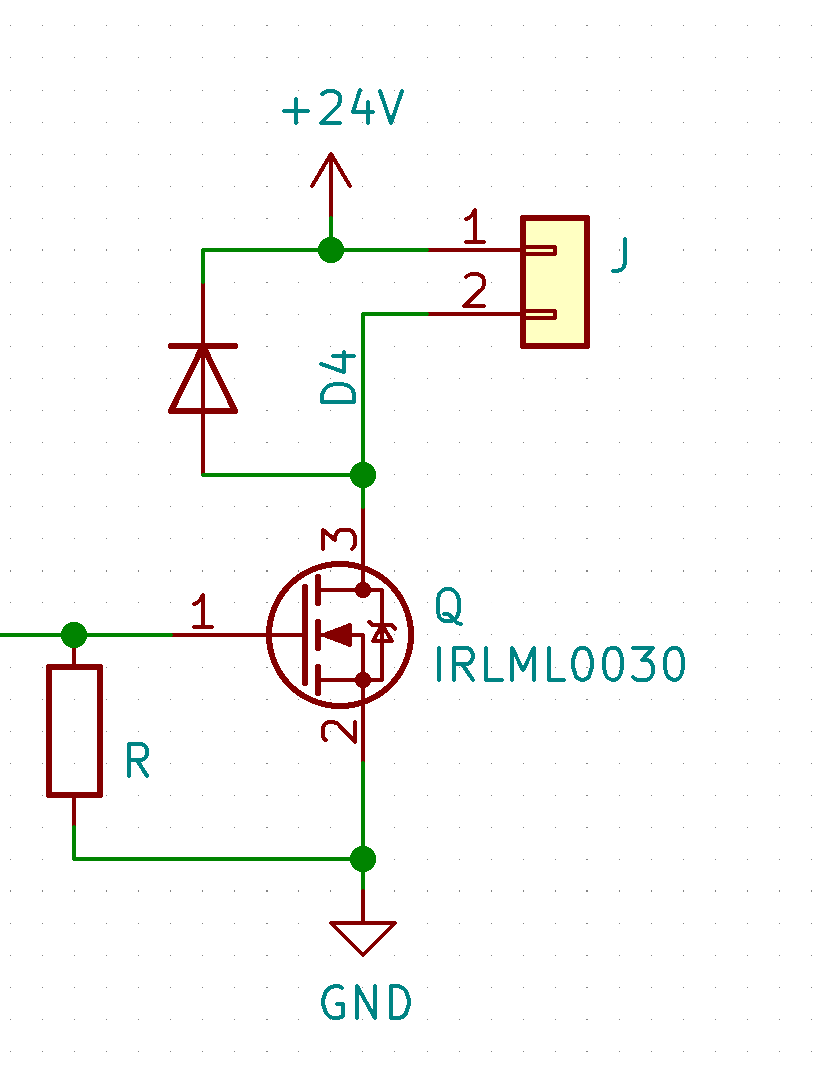
\includegraphics[width=0.7\textwidth]{src/img/circuito_comando.png}
  \caption{Circuito di comando}
  \label{fig:circuito}
\end{figure}
Per quanto riguarda le dimensioni del circuito stampato risultano contenute nonostante la quantità di dispositivi ad esso collegati, infatti il circuito integra solamente la parte composta da una morsettiera con 10 connettori, dedicati ad ognuno degli ingressi necessari, i circuiti di comando e i morsetti di uscita. Ogni circuito di comando è composto un MOSFET e un diodo: 
\begin{description}
\item[Diodo] La funzione del diodo in questo circuito è quella di proteggere il MOSFET e l'uscita di Arduino da sovratensioni indesiderate provocate dagli avvolgimenti presenti nelle elettrovalvole e nei motori, in alcuni casi viene inserito anche per evitare le inversioni di tensione. Per quanto riguarda il circuito di comando per il motore della lama monofase $\SI{230}{\volt}$, utilizzato per la sega, si è preferito introdurre anche un relè così da permettere di utilizzare un MOSFET con corrente di sollecitazione minore e ridurre la tensione massima presente sulla scheda da $\SI{230}{\volt}$ AC a $\SI{24}{\volt}$ DC.
\item[MOSFET] È il cuore del circuito infatti, grazie ad una piccola sollecitazione ($\SIrange{0}{10}{\milli\ampere}$) riesce a veicolare correnti di valore molto più alte ($\SIrange{1}{7}{\ampere}$), nel nostro caso le correnti non superano normalmente i $\SI{2}{\ampere}$ quindi, date le correnti basse non necessitano della presenza di alette di raffreddamento. Per quanto riguarda invece il motore responsabile della movimentazione dell'asse lineare necessita di $\SI{7,7}{\ampere}$ come corrente di spunto.
\end{description}
\section{Quadro}
La seconda parte del circuito è racchiusa in un quadretto di modeste dimensioni al quale viene data in ingresso una tensione monofase $\SI{230}{\volt}$ e in uscita due tensioni continue dal valore di $\SI{24}{\volt}$ e $\SI{12}{\volt}$.
Per permettere la conversione in tensione continua sono stati creati due circuiti di trasformazione separati e provvisti di interruttori magnetotermici differenziali per garantire la sicurezza elettrica del quadro.
Il quadretto in questione verrà in seguito collegato al connettore di terra dello stabilimento.
\section{Descrizione della componentistica}
Sono stati utilizzati i seguenti componenti:
\begin{itemize}
\item Motore dell'asse lineare: un motore brushless di Pamoco con dati di targa di $\SI{24}{\volt}$ e corrente di spunto di $\SI{7,7}{\ampere}$;
\item Motore della sega circolare: un motore di Bonfiglioli con dati di targa di $\SI{230}{\volt}$ monofase e corrente di spunto di $\SI{2,4}{\ampere}$;;
\item Elettrovalvola 4/2 di Fluidmec con pilotaggio elettrico su entrambi i lati con dati di targa di $\SI{24}{\volt}$ e corrente di spunto di $\SI{0,8}{\ampere}$; 
\item Elettrovalvola 5/3 di Festo a centri chiusi con pilotaggio elettrico su entrambi i lati con dati di targa di $\SI{24}{\volt}$ e corrente di spunto di $\SI{0,5}{\ampere}$;
\item Elettrovalvola 3/2 di Schmieranlagen con pilotaggio elettrico a sinistra e ritorno a molla a destra con dati di targa di $\SI{24}{\volt}$ e corrente di spunto di $\SI{0,8}{\ampere}$;
\end{itemize} 

\chapter{Programmazione}
\section{Programma Arduino}
L'intero sistema è basato sulla piattaforma open source \emph{Arduino MEGA}, la quale gestisce l'intero funzionamento del sistema. Il programma che gira su Arduino è basato su un sistema a task e scheduler, ciò vuol dire che l'intero programma è suddiviso in piccoli sottoprogrammi (task) che vengono eseguiti ad una certa frequenza predefinita dallo scheduler il quale compito è appunto quello di eseguire questi programmi al momento giusto. Il programma dispone anche di un sistema per verificare se il sistema è real-time, ovvero che la capacità di calcolo del microcontrollore sia adeguata alla mole di calcoli richiesti dal programma. Questo sistema verifica appunto la saturazione della CPU.
\subsection{SFC}
Il programma per la movimentazione viene eseguito da un task adibito al corretto funzionamento dove si è cercato di replicare un sistema a stati.
\begin{enumerate}
\item Stato di STOP;
\item Tutte le movimentazioni vengono calibrate, quindi tutti i pistoni tranne 2M1 vengono resettati e l'asse lineare si sposta nella posizione più lontana dalla lama;
\item Viene pinzato il tubo con il pistone 1M1;
\item Viene resettato il pistone 2M1 e l'asse lineare si sposta in avanti verso la lama. Se la lunghezza del tubo non è soddisfatta si torna al punto 2;
\item Il tubo viene pinzato con il pistone 2M1;
\item Viene accesa la lama e viene effettuato il taglio con 3M1;
\item Viene fermata la lama e viene retratto il blocco di taglio con 3M2;
\item Viene espulso il pezzo finito e si torna allo stato di calibrazione.
\end{enumerate}
\section{Sistema asse lineare}
È stato deciso di studiare in profondità il funzionamento dell'asse lineare per poter tarare con maggior accuratezza il controllore. È quindi necessario conoscere le specifiche sia del motore che dell'asse lineare:
\begin{table}[H]
\centering
\begin{tabular}{|l|c|c|}
  \hline
\textbf{Descrizione}    & \textbf{Sigla} & \textbf{Valore}   \\ \hline
  \multicolumn{3}{|c|}{\textbf{Dati Motore}}                                                               \\ \hline

Corrente di spunto      & $i_s$                              & \SI{7,7}{\ampere}                       \\ \hline
Tensione nominale       & $v_n$                              & \SI{24}{\volt}                          \\ \hline
Velocità motore a vuoto & $\omega_{n}$                       & \SI{3500}{\rpm}                          \\ \hline
\multicolumn{3}{|c|}{\textbf{Dati asse lineare}}                                                         \\ \hline
Momento di inerzia      & $J$                                & \SI{0,11}{\kg\cm\squared\per\m} \\ \hline
Passo vite              & $p$                                & \SI{5}{\mm}                         \\  \hline
\end{tabular}
\end{table}
È necessario inoltre calcolare la resistenza di armatura e la costante elettrica e meccanica del motore:
\begin{equation}
  R_a=\frac{v_n}{i_s}=\SI{3,12}{\ohm}
\end{equation}
\begin{equation}
  K=\frac{v_n}{\omega_n}=\SI{6,86}{\milli\volt\per\rpm}
\end{equation}
\subsection{Sistema motore}
Per poter studiare il motore si fa uso delle formule del motore in corrente continua:
\begin{equation}
  \begin{cases}
    Ri(t)+K\omega(t)=V(t)\\
    J\dot \omega(t)=Ki(t)
  \end{cases}
\end{equation}
Si decide quindi di portare l'intero sistema nel dominio di Laplace:
\begin{equation}
  \begin{cases}
    RI(s)+K\omega(s)=V(s)\\
    Js\omega(s)=KI(s)    
  \end{cases}
\end{equation}
Eliminando $I(s)$ si ottiene:
\begin{equation}
  \frac{Js\omega(s)}{K}=\frac{V(s)-K\omega(s)}{R}\longrightarrow\frac{\omega(s)}{V(s)}=\frac{K}{JsR+K^2}
\end{equation}
\subsection{Sistema completo}
Dopo aver trovato la funzione che descrive il funzionamento del motore CC è necessario anche descrivere il funzionamento del controllore. Nel nostro caso è stato utilizzato un controllore PID. Lo schema a blocchi rappresenta il sistema completo:
\begin{figure}[H]
  \centering
  \begin{tikzpicture}[auto, node distance=3cm,>=latex']
    \tikzstyle{block} = [draw, rectangle, 
    minimum height=3em, minimum width=6em]
    \tikzstyle{sum} = [draw, circle, node distance=1cm]
    \tikzstyle{input} = [coordinate, node distance=1cm]
    \tikzstyle{output} = [coordinate, node distance=2cm]
    \tikzstyle{pinstyle} = [pin edge={to-,thin,black}]
    
    \node [input, name=input] {};
    \node [sum, right of=input] (sum){};
    \node [block, right of=sum] (controller) {Controller};
    \node [block, right of=controller] (motore) {Motore};
    \node [block, right of=motore] (conversione) {Conversione};
    \node [output, right of=conversione] (output) {};

    \draw [draw,->] (input) -- node {$S_p$} (sum);
    \draw [->] (sum) -- node {$e$} (controller);
    \draw [->] (controller) -- (motore);
    \draw [->] (motore) -- (conversione);
    \draw [->] (conversione) -- node [name=y] {$y$}(output);
    \draw [->] (y) |- (5,-2) -| (sum);
    \node [below left] at (sum) {$-$};
  \end{tikzpicture}
\end{figure}
A questo punto avendo la descrizione del sistema completo si è deciso di simulare l'intero sistema tramite l'utilizzo di Octave. Il risultato sottostante si è ottenuto con $K_P=2$ e $K_I=K_D=0$.
\begin{figure}[H]
  \centering
  \includegraphics[width=0.7\textwidth]{src/img/pid_controller.eps}
  \caption{Simulazione asse lineare}
  \label{fig:simulazione}
\end{figure}
Tarando quindi i giusti valori di PID è possibile ottenere un sistema teoricamente ottimale, ma che richiede comunque una prova sperimentale sul campo.

\chapter{Sviluppi futuri}
\section{Sviluppi ambito elettronico}
  Uno sviluppo futuro per questo progetto consisterebbe nella progettazione e realizzazione di un circuito di sicurezza implementando barriere o cancelli che impediscano agli operatori di infortunarsi a causa delle diverse parti in movimento presenti nel macchinario.

\section{Sviluppi ambito programmazione} 
Sono da implementare l'interfacciamento con l'utente tramite l'utilizzo di un encoder e di un display LCD, nonché la comunicazione seriale con un PC per effettuare un debugging del sistema se necessario. Un'implementazione futura potrebbe consistere nella creazione di un applicativo di visione, magari per il controllo della qualità la deformazione del tubo dopo il taglio.
  
\section{Sviluppi ambito meccanico}  
  Un altra possibile modifica al progetto potrebbe consistere nella creazione di un sistema mobile per quanto riguarda la struttura contenente la sega circolare così da permettere anche quest'ultima di muoversi al posto della sola movimentazione del tubo, ottimizzando così le tempistiche dedicate al taglio.
  Un possibile miglioramento futuro, riferito alla parte meccanica, potrebbe consistere nell’utilizzo di una struttura verticale con la lamiera di supporto per lo scorrimento del tubo a forma di “V”, con relativa rulliera e i pistoni 1M1 e 2M1 (che utilizzano lo stesso sistema di trasporto) disposti al di sopra di quest’ultima. Per la parte di taglio, invece, si pensava di effettuare il taglio mediante una lama circolare calettata ad un piccolo motore elettrico, il tutto fissato a delle piastre montate su un corsoio con relative sicurezze, per movimentare agevolmente un peso contenuto in orizzontale; ed infine per la parte di scarico una lamiera mobile che viene mossa da un pistone per rilasciare il pezzo finito lungo uno scivolo.

\chapter{Crediti}
\section{Software utilizzati}
\begin{description}
\item[Autodesk Inventor]Per la realizzazione e la rappresentazione dei pezzi meccanici
  \item[Fluidsim]Per la progettazione del sistema pneumatico
\item[KiCad]Per la progettazione del PCB
\item[Arduino]Per la programmazione del sistema
\item[Octave]Per la simulazione del sistema
\item[\LaTeX]Per la documentazione
\end{description}
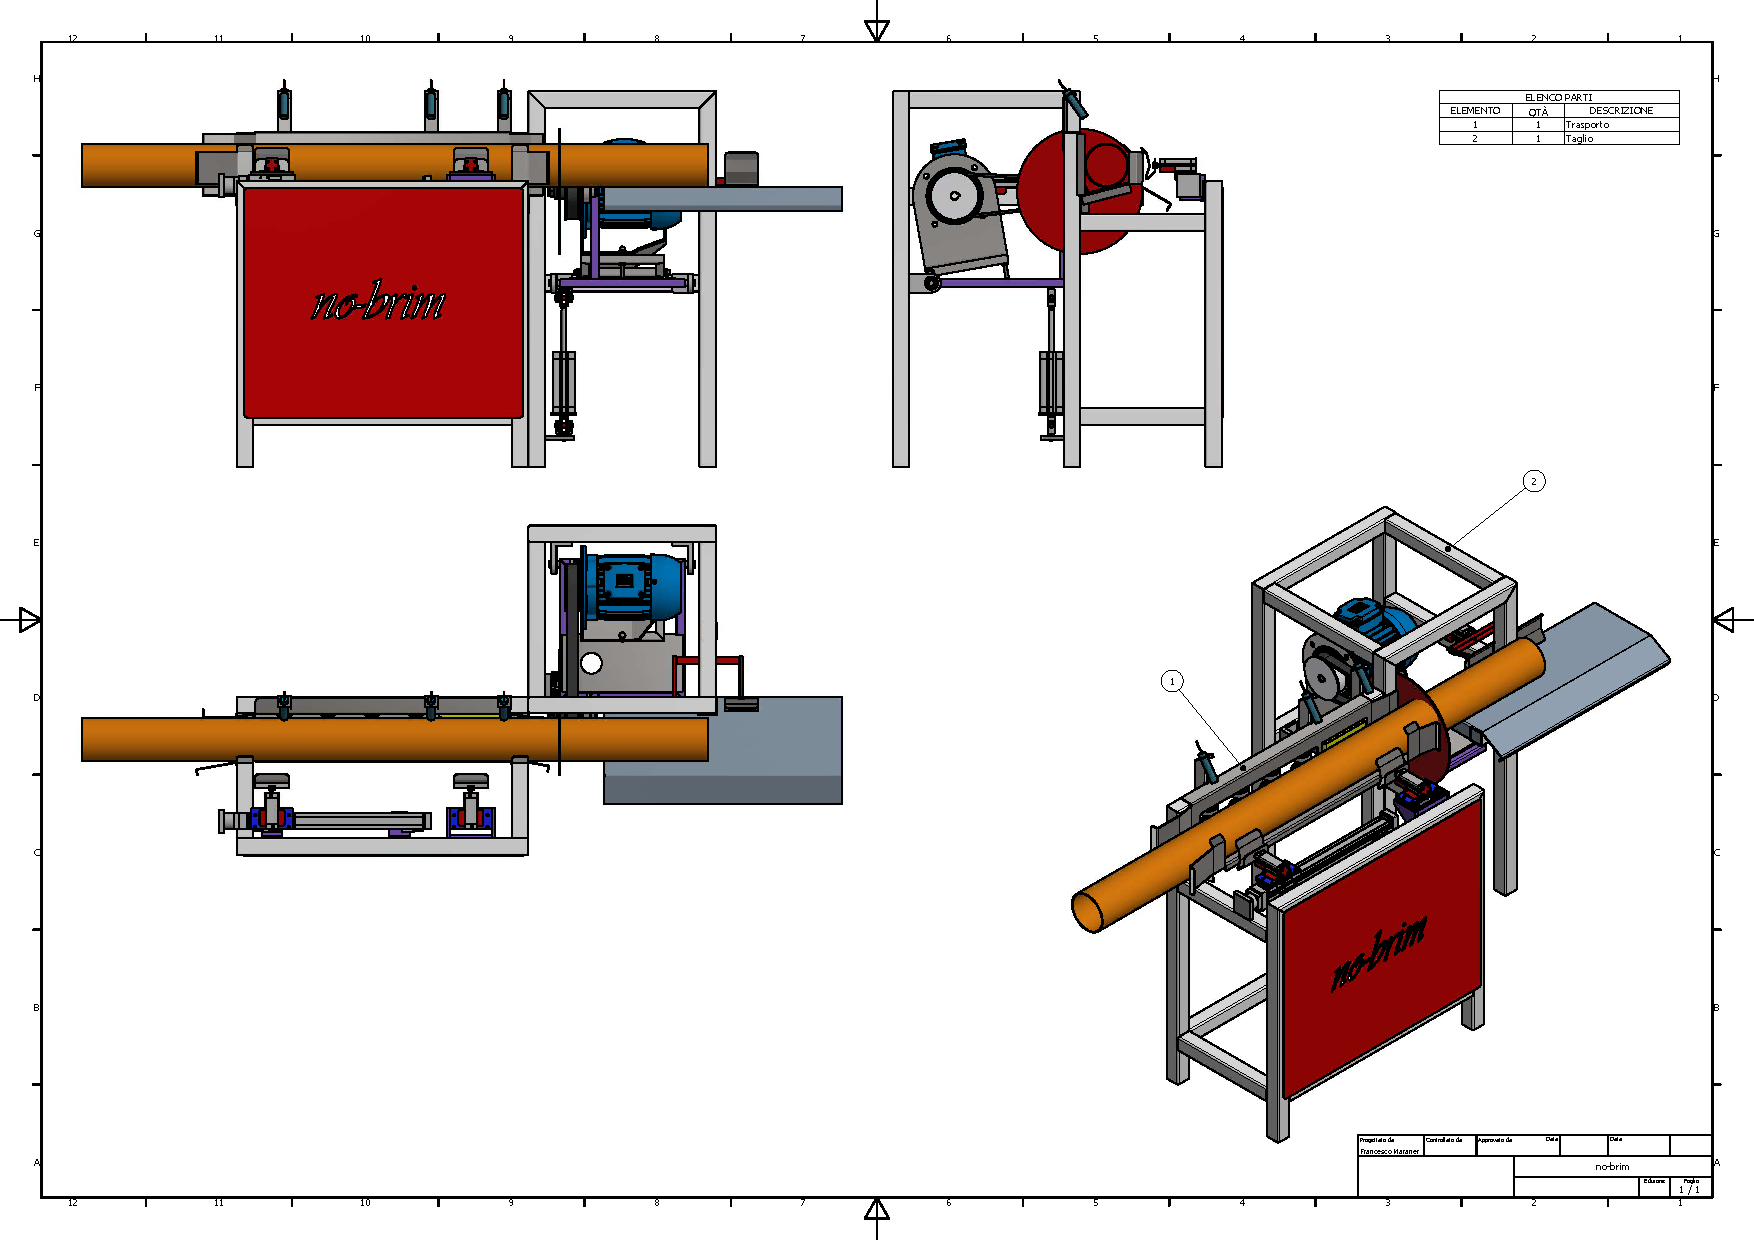
\includepdf[pages=-,angle=90]{src/Tavole/completo.pdf}
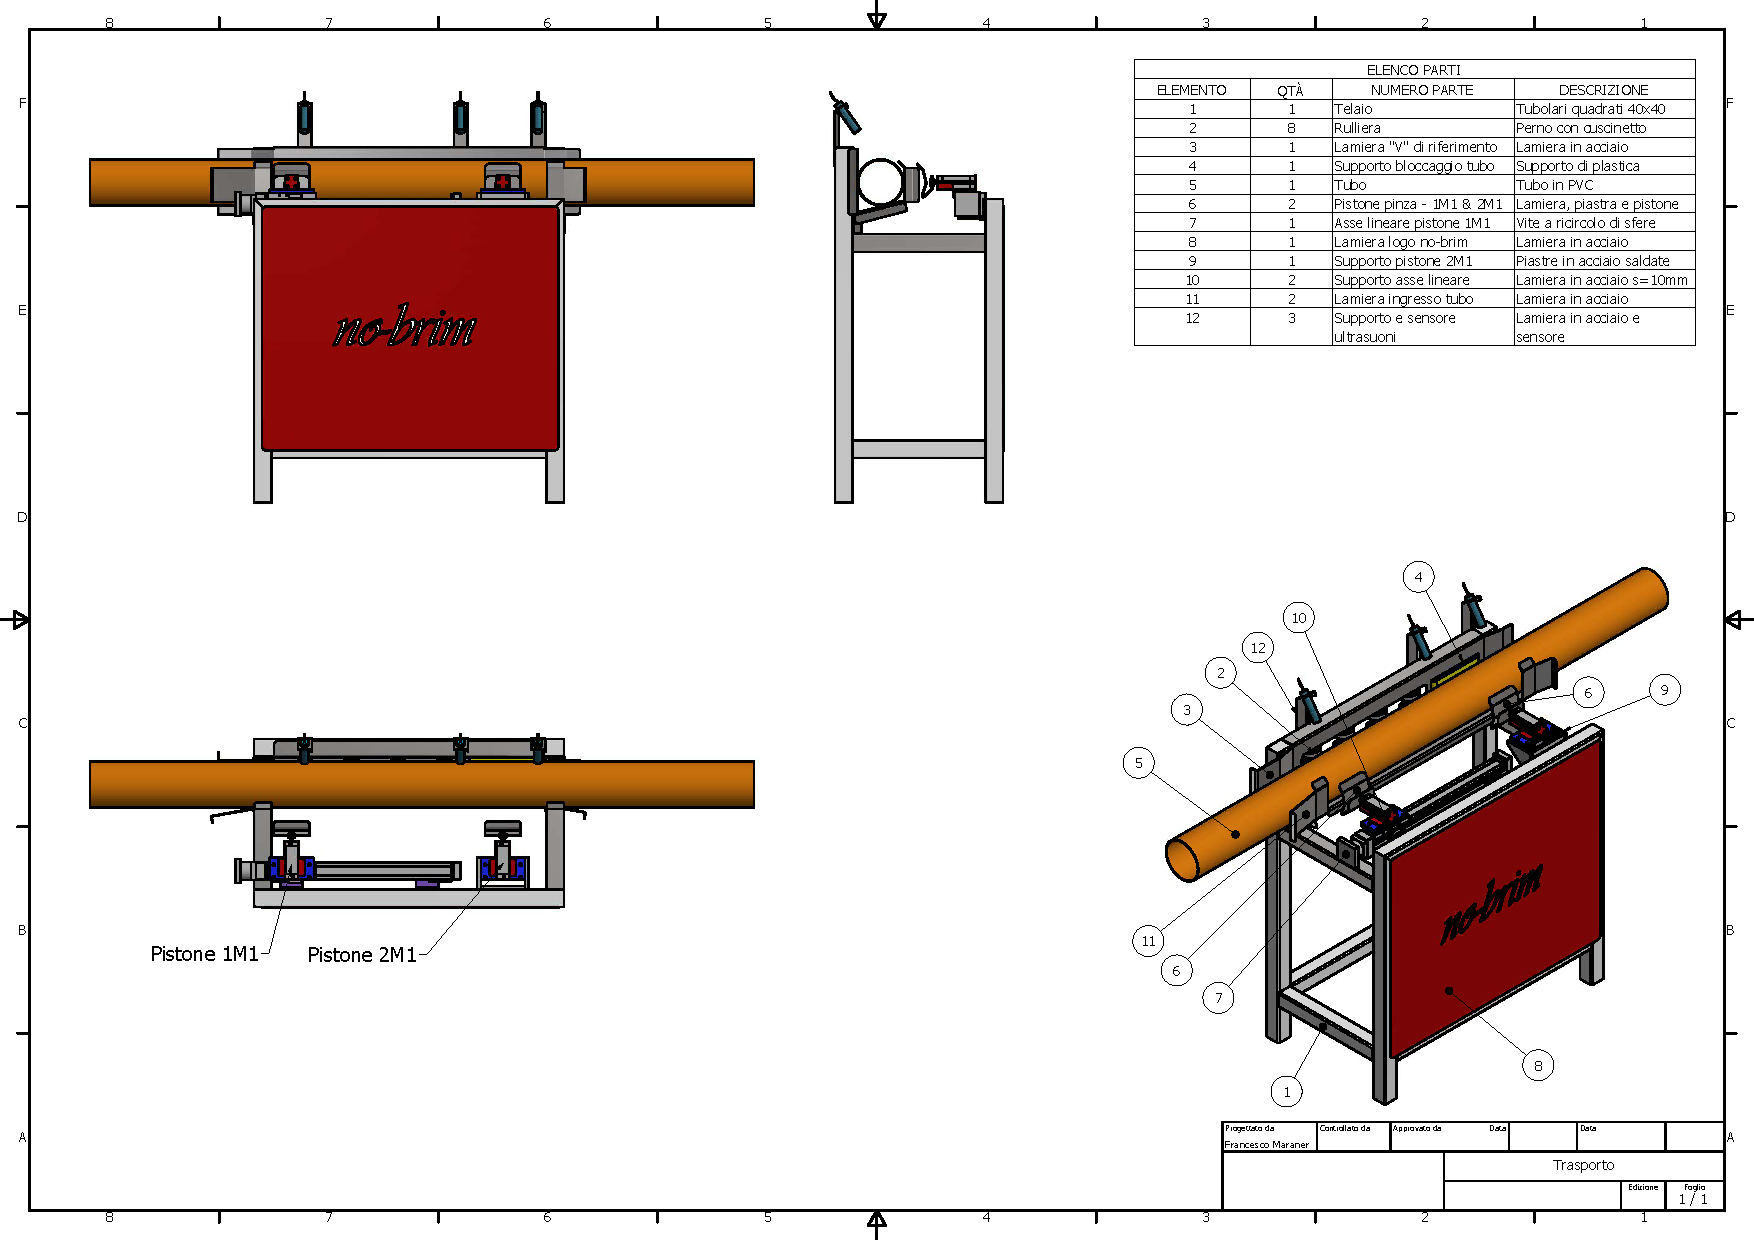
\includepdf[pages=-,angle=90]{src/Tavole/trasporto.pdf}
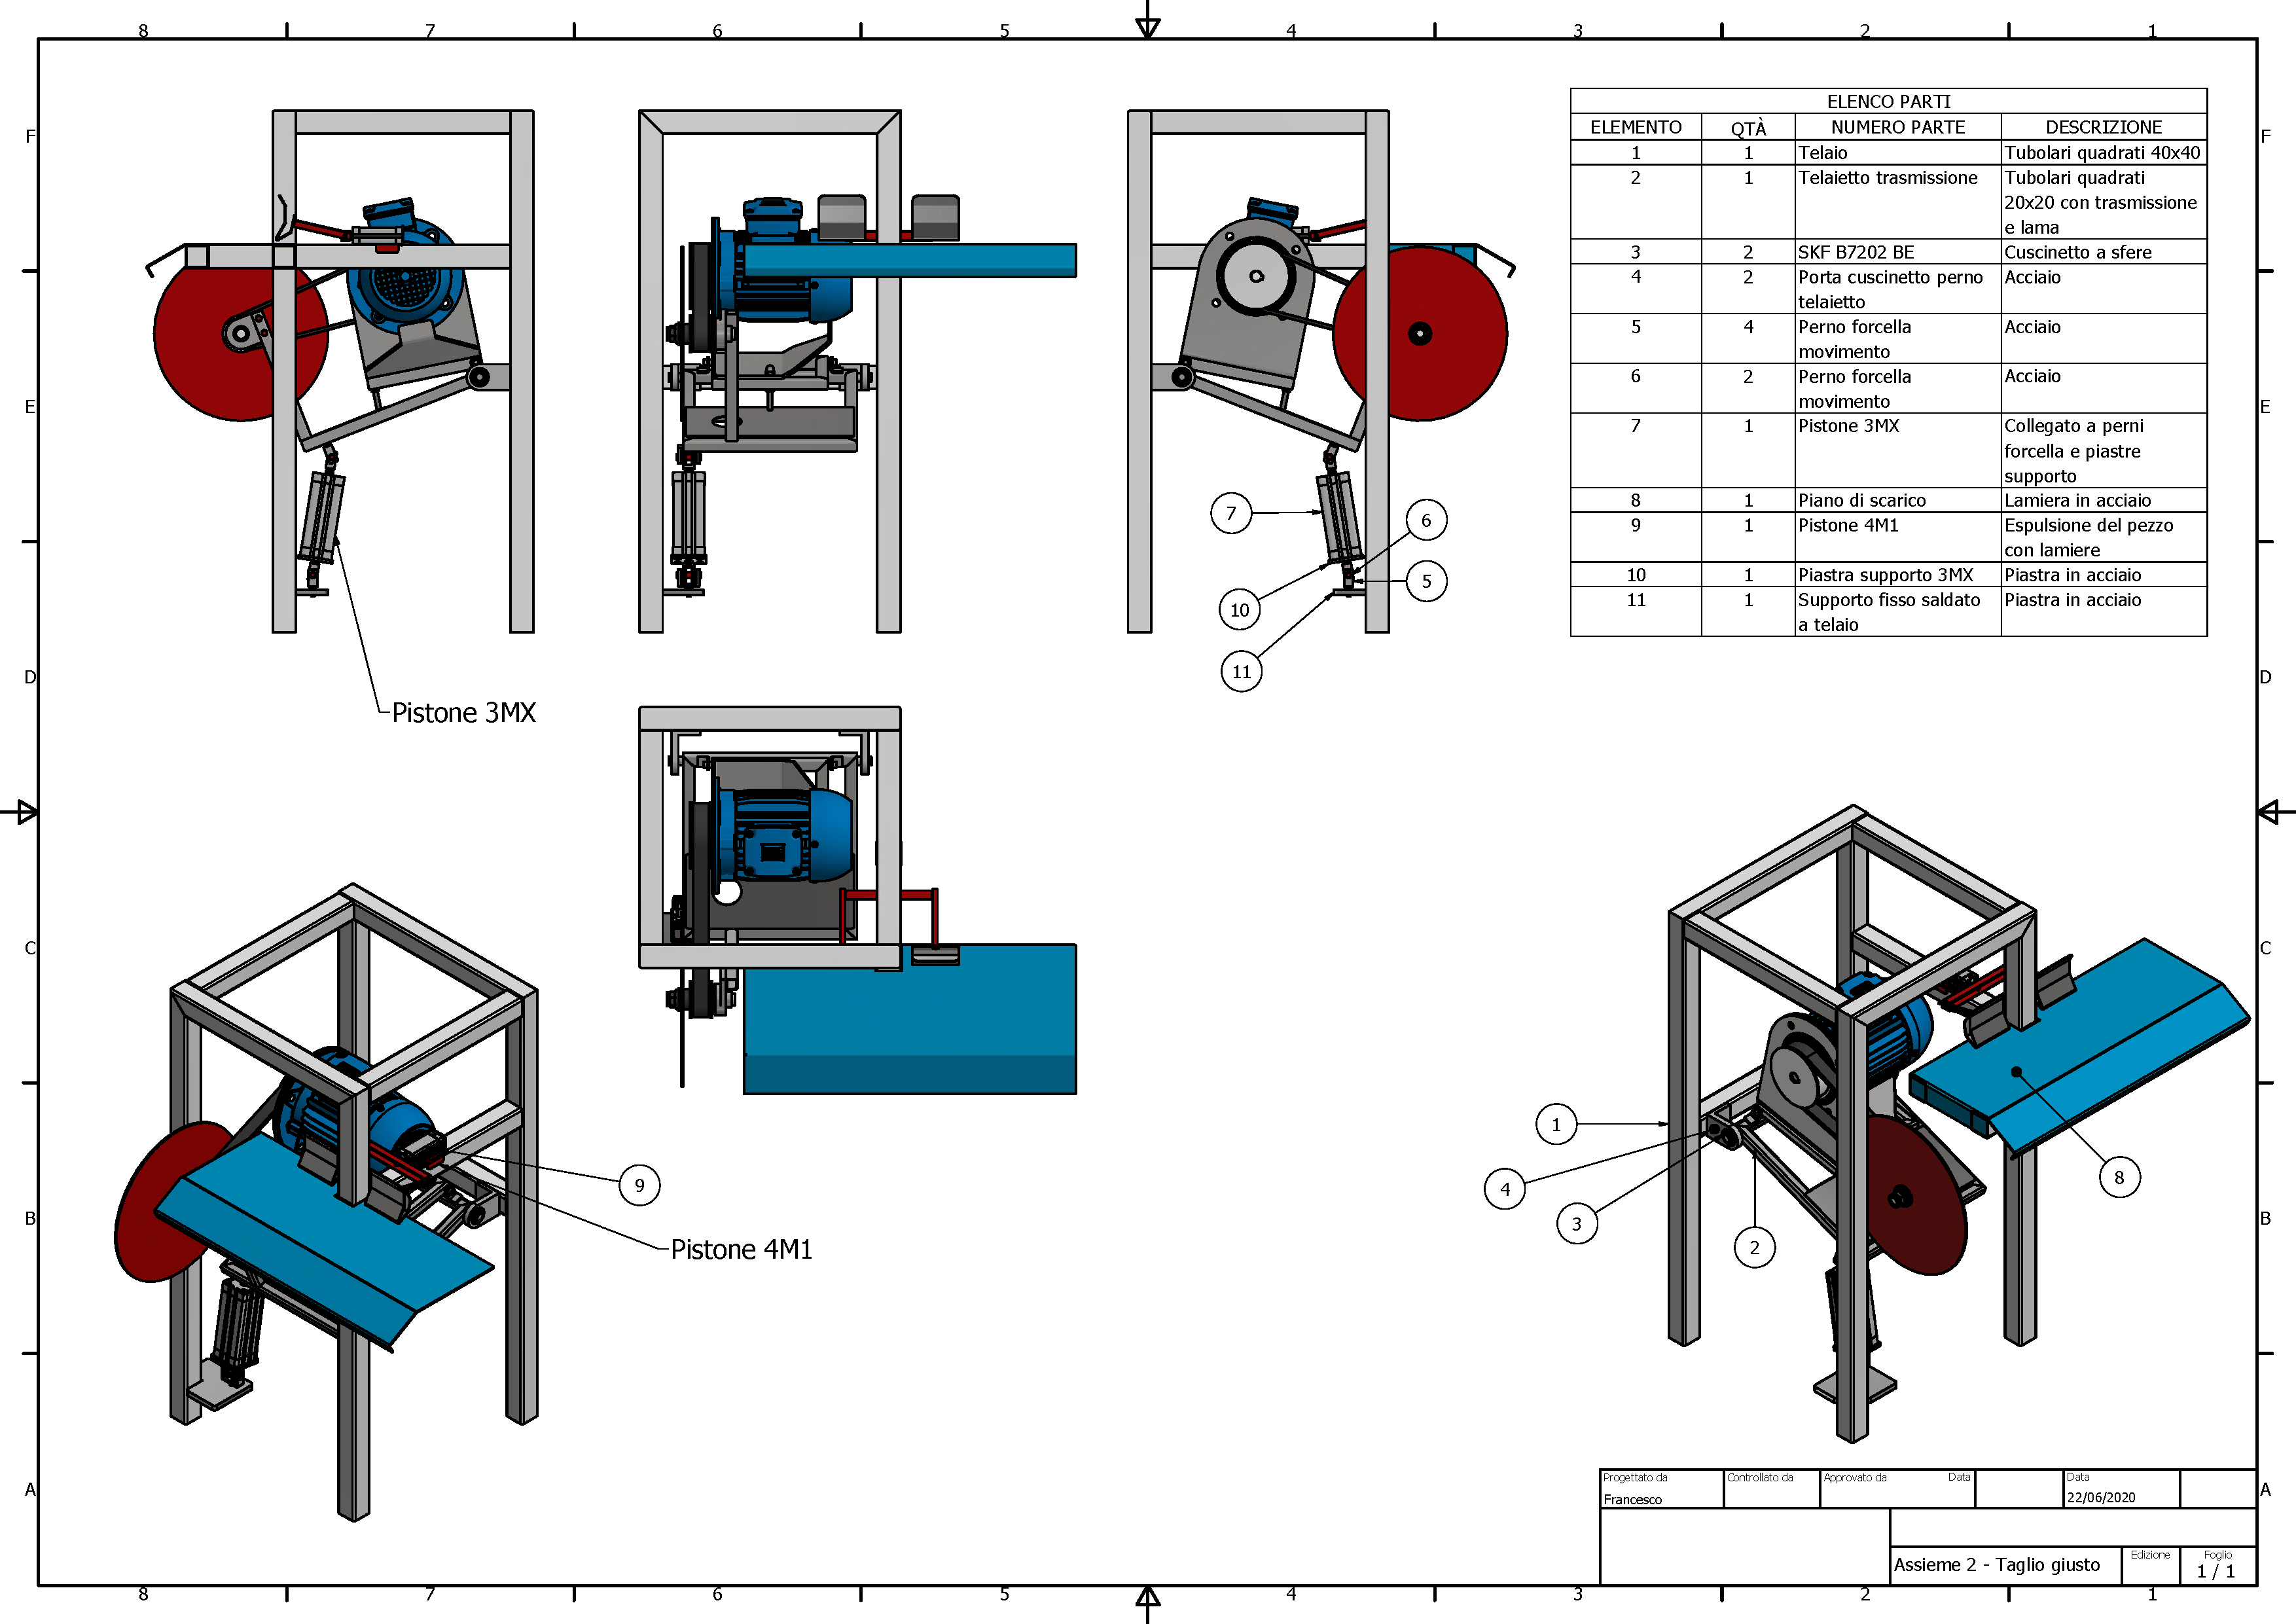
\includepdf[pages=-,angle=90]{src/Tavole/taglio_1.pdf}
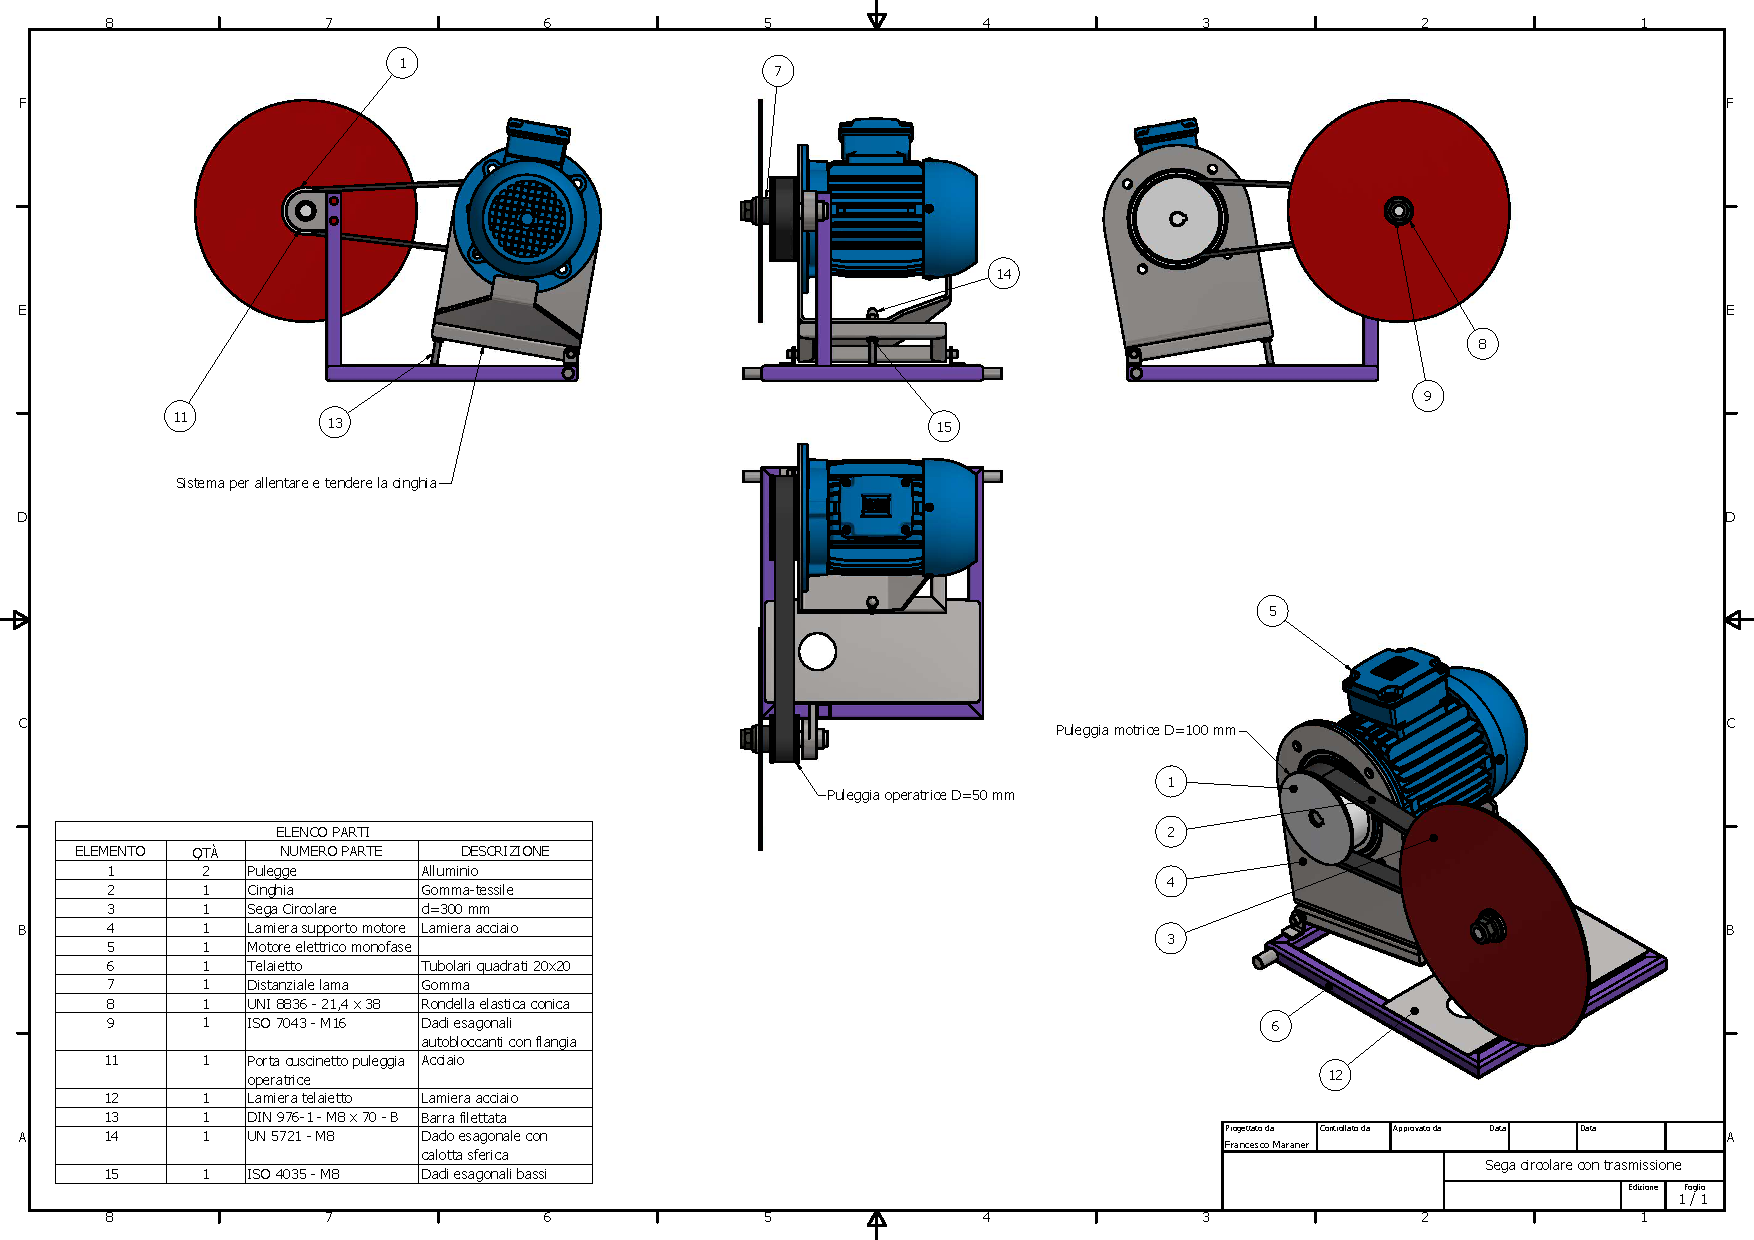
\includepdf[pages=-,angle=90]{src/Tavole/trasmissione.pdf}
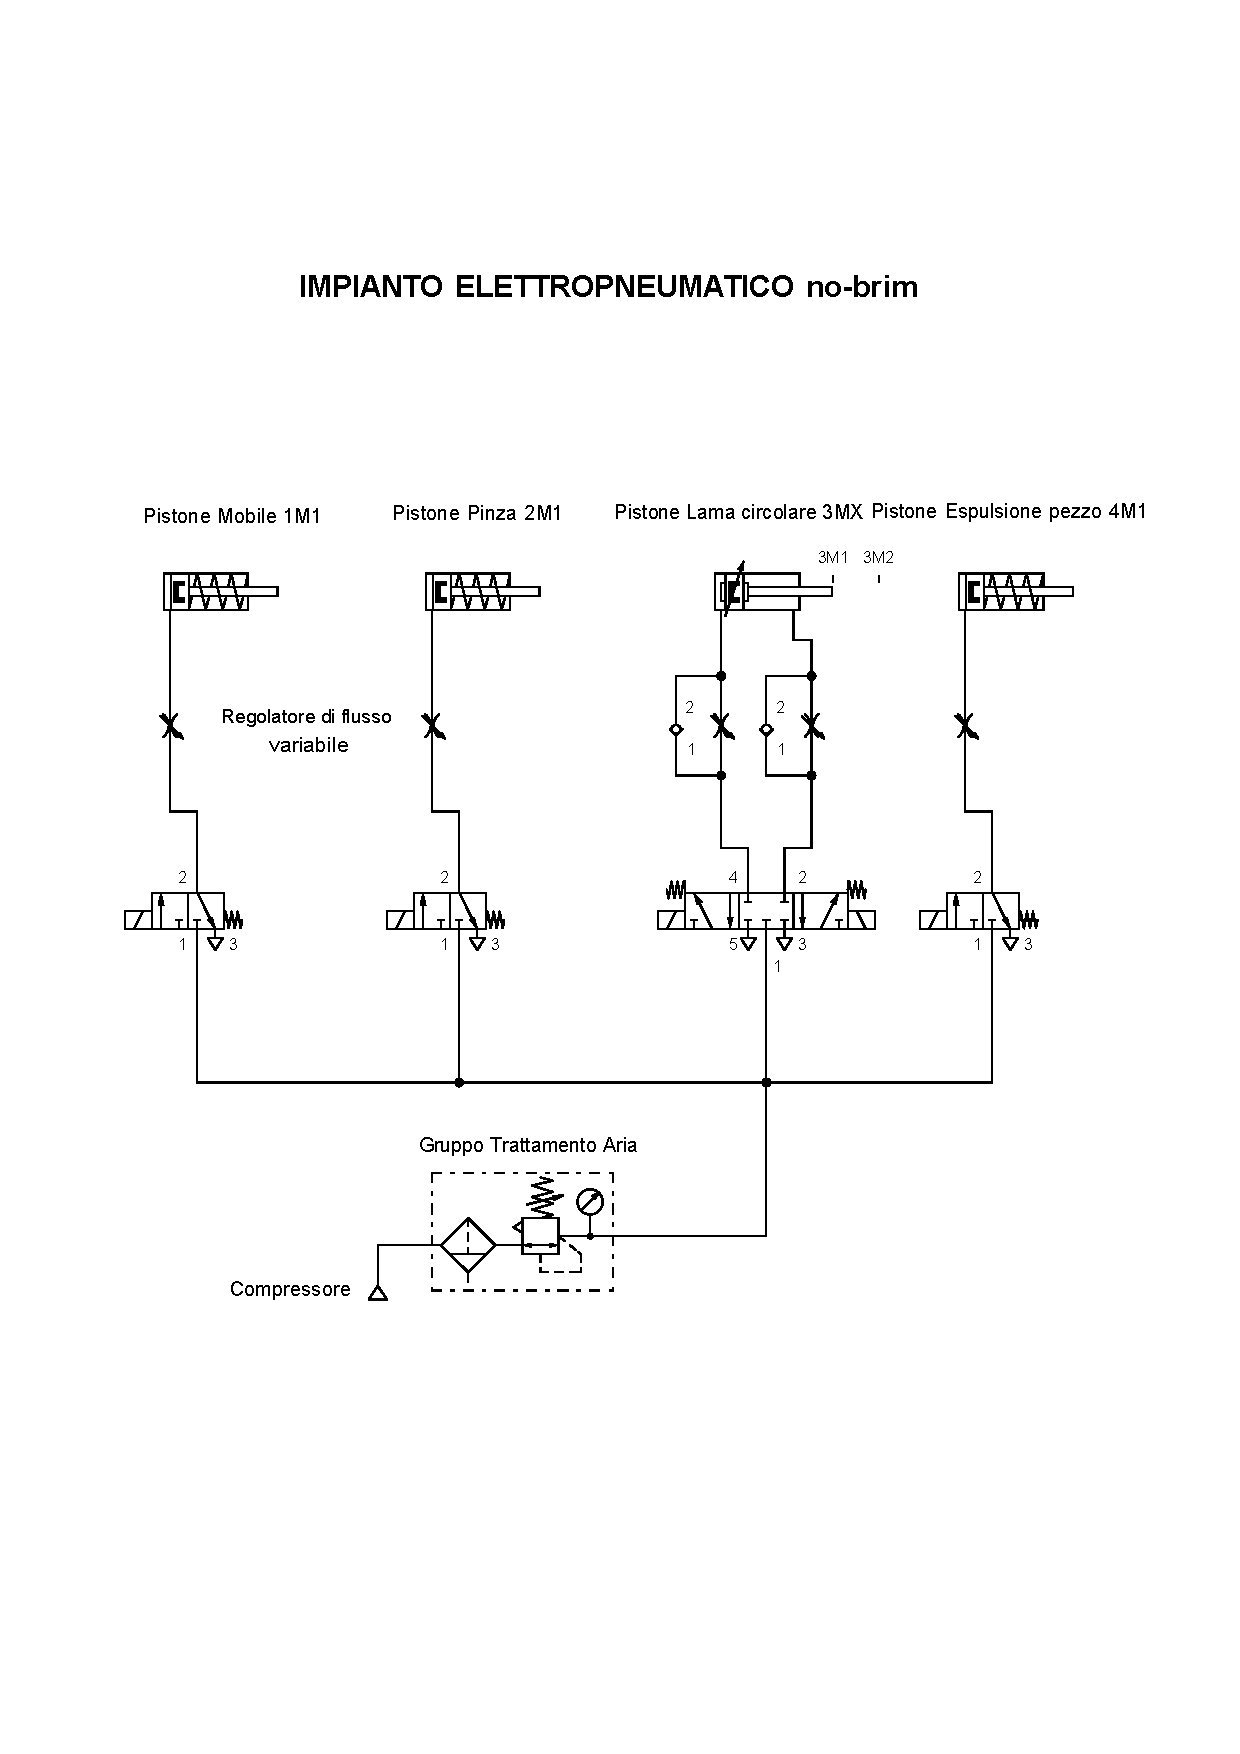
\includepdf[pages=-]{src/img/impianto_elettropneumatico.pdf}
\end{document}
